\section{Algebra}
\label{sec:algebra}
\setlength{\textfloatsep}{5pt}% Remove \textfloatsep

\tg algebra, or \tga for short, is compositional: operators take a \tg
or a pair of \tgs as input, and output a \tg.  We specify the
semantics of \tga by showing a translation of each operator into a
sequence of temporal relational algebra (\tra) expressions (with
nesting, to accommodate non-1NF vertex/edge attributes).  Using this
translation one can implement \tga in a temporal DBMS, guaranteeing
snapshot reducibility and extended snapshot
reducibility~\cite{DBLP:reference/db/Bohlen092} --- two properties
that are appropriate for a point-based temporal data model.

\tra algebra extends relational algebra by specifying how operators
are applied to temporal relations such that snapshot reducibility
property is guaranteed.  Additionally, explicit references to time are
supported in operator predicates (extended snapshot reducibility), but
the time stamps are not manipulated by the user queries directly.

%\julia{TRA refresher: time as data, RA operations implicitly handle
%  time (snapshot reducibility), explicit reference to time are
%  supported in the predicates (extended snapshot reducibility), but
%  time cannot be ``created''.}

%\julia{Explain temporal subset}

In Section~\ref{sec:algebra:integrity} we present the primitives that
are needed to enforce soundness of \tga.  Then, in
Sections~\ref{sec:algebra:unary} through~\ref{sec:algebra:ecreate}, we
present \tga operators.  Section~\ref{sec:analytics} presents an
extension of \tga to support Pregel-style analytics.  \eat{We conclude
  by showing expressiveness of \tga in Section~\ref{sec:aformal}.}

\subsection{Primitives and Soundness}
\label{sec:algebra:integrity}

\tga operators are translated into expressions in temporal relational
algebra (\tra).  Since TRA is applied to individual relations of \tve,
we must ensure that the combined state of these relations in the
result corresponds to a valid \tg, i.e., that the translation is
sound.  Recall from Definition~\ref{def:tg} that a valid \tg must
satisfy four requirements: {\bf R1}: Unique vertices and edges, {\bf
  R2}: Unique attribute values, {\bf R3}: Referential integrity, and
{\bf R4}: Coalesced.  We now describe four primitives that will ensure
soundness of \tga.

{\bf Coalesce.} To enforce requirements {\bf R1} and {\bf R4}, we
introduce the coalesce primitive $\coal{R}$, which merges adjacent or
overlapping time periods for value-equivalent tuples.  This operation
is similar to duplicate elimination in conventional databases, and has
been extensively studied in the
literature~\cite{DBLP:conf/vldb/BohlenSS96,DBLP:journals/sigmod/Zimanyi06}.
$\coal{R}$ is applied to individual relations of \tve, or to
intermediate results, following the application of operations that
uncoalesce.
%
The coalesce primitive can be implemented in relational
algebra~\cite{DBLP:conf/vldb/BohlenSS96}.  If a DBMS supports
automatic coalescing, this primitive is not necessary.

{\bf Resolve.} To enforce {\bf R2} we introduce the resolve primitive
$\resolve{f_1(k_1), \ldots, f_n(k_n)}{R}$, which is invoked by
operations that produce attribute relations with duplicates.  Resolve
computes a temporal group-by of the attribute relation $R$ by key
(e.g., by $v$ if $R$ represents vertex attributes).  It then computes
a bag-union of the properties occurring in each group, groups together
key-value pairs that correspond to the same property name $k_i$, and
aggregates values within each group using the specified aggregation
function $f_i$.  If no aggregation function is specified for a
particular property name, \insql{set} is used as the default.  For
example, if $R$ contains tuples $(v_1, [2/15,4/15),
  \{name=Ann,sal=100\})$ and $(v_1, [2/15, 3/15),
    \{name=Ann,sal=200\})$, the result of $\resolve{AVG(sal)}{R}$ will
    contain $(v_1, [2/15,3/5), \{name=Ann,sal=150\})$ and $(v_1,
      [3/15,4/5), \{name=Ann,sal=100\})$.  The resolve primitive can
        be implemented with temporal relational aggregation $\gamma^T$
        over unnested relations.

{\bf Constrain.} To enforce {\bf R3} we introduce the constrain
primitive $\constr{r}{s}$, which enforces referential integrity on
relation $\mathbf{r}$ with respect to relation $\mathbf{s}$.  For
example, this primitive is used to remove edges from \te for which one
or both vertices are absent from \tv, or validity period of an edge to
be within the validity periods of its vertices.  

{\bf Split.} The final primitive $\wsplit{s}{w}{R}$ uncoalesces
relation $R$ in a particular way.  For each tuple $t \in R$ with time
period $p$, it emits a set of tuples, with the same values for
non-temporal attributes as in $t$, but with time periods split into
windows of width $w$ with respect to start time $s$.  For example,
$\wsplit{2/15}{3~\textsf{months}}{\te}$ for \insql{T1} in
Figure~\ref{fig:tg_ve} produces an uncoalesced relation with 2 tuples
for $(v_1, v_2)$, with periods $[2/15, 5/15)$ and $[5/15, 6/15)$, and
    2 tuples for $(v_2, v_3)$, with validity periods $[7/15, 8/15)$
      and $[8/15, 10/15)$.  This primitive will be necessary to
        express the temporal variant of node creation
        (Section~\ref{sec:algebra:ncreate})\eat{, and is essentially a
          temporal normalization
          method~\cite{DBLP:conf/time/BohlenGJ06}}.  It will be used
        at an intermediate step in the computation, all final results
        will be coalesced as needed, enforcing {\bf R4}.

\eat{The reduce function may, for example, pick the left, the right,
  or an arbitrary element, compute the value of an aggregate function
  such as $\mathbf{COUNT}$, or accumulate values into a set.  A reduce
  function can be repeatedly applied to an unordered collection of
  values to compute a single value, as is done in the map-reduce
  model.  The property graph model allows for arbitrary properties to
  be associated with the graph entities, so it may be impractical or
  infeasible to have the user specify a reduce function for each
  possible property.  In \ql a default reduce function \insql{set} is
  used for any property without an explicitly stated reduction.}

\eat{\begin{lemma}
Let $\psi$ be an n-ary temporal operator on \tg.  If $\psi^T (\ttt)$
produces multiple possible attribute values for any entity at the same
time instant, it must also specify a resolve function for each
property to compute a single valid attribute value.
\end{lemma}}

\eat{In operator definitions below we note which operators are known to
uncoalesce the output, thus requiring coalescing, require FK
enforcement, or include reduce functions.  All non-trivial proofs are
listed in Appendix~\ref{sec:app1}.}

\subsection{Unary operators}
\label{sec:algebra:unary}

{\bf Slice.} The slice operator, denoted $\slice{\bc}{\ttt}$, where
$\bc$ is a time interval, cuts a temporal slice from \ttt. The
resulting \tg will contain vertices and edges whose period $\bp$ has a
non-empty intersection with $\bc$.  We translate this \tga operator to
TRA statements over each constituent relation of \tve:
$\slice{\bc}{\tv}$ and similarly for \te, \tav and \tae.

%: $\slice{\bc}{\tv} = \{ (v, \bp \cap \bc)~~|~~(v, \bp) \in \tv
%\wedge (\pred{\bc}{overlaps}{\bp} \vee \pred{\bc}{contains}{\bp})
%\}$, and analogously for each \te, \tav and \tae.  apply select
%operator to each of the four constituent relations of \tve: $\forall
%x \in \{\tv,\te,\tav,\tae \}, x' = \pi_{A,p \cap c}(\sigma_{p \cap c}
%(x))$, where $A$ is the non-temporal schema of $x$.

\eat{If $p.start < c.start$ or $p.end > c.end$ for some tuple $(g,
  p)$, then $p$ is trimmed to be within the boundaries of $c$: $\tau_c
  (\trg) = \{ (g, p \cap c)~~|~~(g, p) \in \trg \wedge
  (\pred{c}{overlaps}{p} \vee \pred{c}{contains}{p})\}$.  }

%Slice does not violate any of the soundness requirements {\bf R1} ---
%{\bf R4}. \eat{, see Appendix~\ref{sec:app1} for proofs of this and
%  similar statements.}

{\bf Subgraph.} Temporal subgraph matching is a generalization of
subgraph matching for non-temporal graphs~\cite{Wood2012}.  This query
comes in two variants.

\eat{A temporal vertex-subgraph query $q^T_v(\tve)$ is a conjunctive query
that takes $\tve (\tv, \te, \tav, \tae)$ as input, and outputs
$\tve'$, an induced temporal subgraph of \tve in which vertices are
defined by $q^T_v$.}

Temporal vertex-subgraph \subv{q^t_v}{\ttt} computes an induced
subgraph of \tve $\tve'(\tv', \te', \tav', \tae')$, with vertices
defined by the temporal conjunctive query (TCQ) $q^t_v$.  Note that
this is a subgraph query, and so $\tv' \subseteq^T \tv$.

\eat{A temporal edge-sugraph query $q^t_e(\tve)$ is a conjunctive query
that takes a graph $\tve (\tv, \te, \tav, \tae)$ as input, and outputs
a \tg $\tve'$ on the vertices of $\tve$ such that the edges of $\tve'$
are defined by $q^t_e$. }

Temporal edge-subgraph \sube{q^t_e}{\ttt} computes a subgraph of \ttt
$\tve'(\tv', \te', \tav', \tae')$ in which edges are defined by TCQ
$q^t_e$.  Since this is a subgraph query, $\te' \subseteq^T \te$.

Queries $q^t_v$ and $q^t_e$ may use any of the constituent relations
of \tve, and may explicitly reference temporal information, and so
require all input relations to be
coalesced~\cite{DBLP:reference/db/Bohlen09}.

Following the computation of $\tv' = q^t_v(\tv)$, \subv{q^t_v}{\ttt}
must invoke $\coal{\tv'}$ to enforce {\bf R1} and {\bf R4}; and
$\constr{\te'}{\tv'}$, $\constr{\tav'}{\tv'}$, $\constr{\tae'}{\te'}$
to enforce {\bf R3}.
%
Following the computation $\te' = q^t_e(\te)$, \sube{q^t_e}{\ttt} must
invoke $\coal{\te'}$ to enforce {\bf R1} and {\bf R4}; and
$\constr{\tae'}{\te'}$ to enforce {\bf R3}.  %No further
%validation is required, provided that $q^t_e$ outputs a temporal
%subset of \te.% (see Appendix~\ref{sec:app1}).

\eat{We focus on functions that can be expressed as a pair of {\em
  conjunctive queries} $\sigma_{C_V,C_E} (\ttt)$, where $C_V$
specifies a predicate over the vertices and $C_E$ --- over the
vertex-edge triplets.  The predicates can be over the attributes, ids,
and the timestamps of the vertices and edges.  We allow predicates
over the timestamps to support extended snapshot reducibility.
Computing arbitrary subgraphs with path expressions is beyond the
scope of this paper, and we defer this to future work.}

\eat{
$\sigma_{C_V,C_E} (\ttt) = (\tv',\te',\tav',\tae') ~|~$ \\
$\tv' = \pi_{v,p} (\sigma_{C_V} ( \tv \bowtie^T_v \tav))$ \\
$\te' = \pi_{v_1,v_2,p} (\sigma_{C_E} ( \tae \bowtie^T_{v_1} \tav \bowtie^T_{v_2} \tav))$ \\
$\tav' = \sigma_{C_V} (\tav)$ \\
$\tae' = \pi_{v_1,v_2,a} (\sigma_{C_E} (\tae \bowtie^T_{v_1} \tav \bowtie^T_{v_2} \tav))$}

\eat{ Note that as B{\"{o}}hlen showed
  in~\cite{DBLP:reference/db/Bohlen09}, correctness of a select
  operator with a temporal predicate depends on the coalesced state of
  the relation.  When composing a triplet, we carry the vertex and
  edge timestamps in their entirety as data to produce correct
  results.}

% There is no need for an example here, it is clear what these queries
% compute.

\eat{Because we allow predicates over the triplets, interesting conditions
can be expressed.  For example, we can filter out any edges where the
value of some property of its two vertices does not match.  Assuming
vertices have property \insql{group}, we can compute
$\sigma_{T,v1.a.group=v2.a.group}(\ttt)$.}

\eat{
Vertex-subgraph: {\bf R1,R2}: coalesce $\tv'$; {\bf R3}: enforce FK on
$\tav', \te', \tae'$. Edge-subgraph: {\bf R1,R2}: coalesce $\te'$;
{\bf R3}: enforce FK on $\te'$ and $\tae'$.}

\eat{Vertex-subgraph requires coalescing of $\tv'$ and FK enforcement on
\tav', \te', and \tae'. Edge-subgraph requires coalescing of $\te'$ and
FK enforcement on \tae'.}

%\subsection{Temporal map}
%\label{sec:algebra:project}

{\bf Map.}  Temporal vertex-map and edge-map apply user-defined map
functions $f_v$ and $f_e$ to vertex or edge attributes.  Temporal
vertex-map $\vmap{f_v, \tve}$ outputs $\tve'$ in which $\tv'=\tv$,
$\te'=\te$, $\tae' = \tae$, and $\tav' =
\pi^T_{v,f_v(a)}\tav$. Temporal edge-map $\emap{f_e, \tve}$ is defined
analogously.

\eat{To evaluate $\map_{M_V,M_E} (\tve)$, we set $\tv'=\tv$ and $\te'=\te$,
and compute $\tav' = \map_{M_V}(\tav)$ and $\tae' = \map_{M_E}(\tae)$.}

\eat{Temporal map iterates over the tuples of \trg, and applies the
user-specified map functions $M_V$ and $M_E$ to the vertices and edges
of each $g$: $\map_{M_V,M_E} (\trg) = \{(g', p)~~|~~(g,p) \in \trg
\wedge g'= \map_{M_V,M_E}(g)\}$.
}  

While $f_v$ and $f_e$ are arbitrary user-specified functions, there
are some common cases.  Map may specify the set of properties to
project out or retain, it may aggregate (e.g., \insql{COUNT}) or
deduplicate values of a collection property, or flatten a nested
value.
%
To produce a valid \tg, $\vmap{f_v, \tve}$ must invoke $\coal{\tv'}$
and $\emap{f_e, \tve}$ must invoke $\coal{\te'}$.

% because this is an arbitrary operation, we don't need to invent
% syntax here.  it's also clear what this operation does, I don't
% think there is a need for an example.

\eat{In such cases we will use short-hand
notation similar to projection, listing the properties that we wish to
retain. For example, $\map_{M_V:{school},M_E:\emptyset} (\insql{T1})$
will keep only the school property of the vertices, and no properties
of the edges.  Another useful map operation eliminates duplicates in
the bag of a particular vertex or edge property.  \eat{It may also be
useful to flatten nested bags or aggregate multiple values of the same
property of a vertex or edge, e.g., compute a sum or an average
following temporal intersection or union
(Section~\ref{sec:algebra:join}).}}

%Vertex-map: {\bf R2}: coalesce $\tav'$.  Edge-map: {\bf R2}: coalesce
%$\tae'$.

\eat{Vertex-map requires only coalescing of $\tav'$. Edge-map requires
  only coalescing of $\tae'$.}

\subsection{Aggregation}
\label{sec:algebra:agg}

Aggregation is a common graph operation that computes the value of a
vertex property $pname$ based on information available at the vertex
itself, at the edges associated with the vertex, and at its immediate
neighbors.  Aggregation can be used to compute simple properties such
as in-degree of a vertex, or more complex ones such as the set of
countries in which the friends of $v$ live.

It is convenient to think of aggregation as operating over a temporal
view $L(v_1,v_2,v_1.a,v_2.a,e.a,p)$, where $v_1$ refers to the vertex
for which the new property is being computed, $v_2$ refers to the
vertex from which information is gathered, $v_1.a$, $v_2.a$ and $e.a$
are attributes of the vertices and of the edge, and $p$ is the
associated time period.  $L$ is computed with a temporal join of \te
with two copies of \tv, one for each side of the edge, and with $\tav$
and $\tae$ outer-joined with the corresponding relations.  Outer-joins
are needed because a vertex / edge is not required to specify an
attribute.

When \tve represents a directed graph, direction of the edge can be
accounted for in the way the join is set up (e.g., mapping $v_2$ in
\te to $v_1$ in $L$ if the goal is to aggregate information on
incoming edges).  When \tve represents an undirected graph (recall
that we choose a canonical representation of an edge, with $v_1 \leq
v_2$), or when direction of the edge is unimportant, $L$ can be
computed from $\te(v_1,v_2,p) \cup^T \te(v_2,v_1,p)$ rather than from
$\te$.

Aggregation is denoted $\insql{agg}^T(dir,cond,f_m,f_a,pname,\ttt)$,
where $dir$ is the direction of the edge (one of 'right', 'left' or
'both') that determines how $L$ is computed, $cond$ is a predicate
over $L$, $f_m$ is a map function that emits a value for each tuple in
the result of $\sigma^T_{cond}(L)$ (e.g., 1 for computing degree of
$v_1$, or $v_2.a.country$ for computing the set of countries in which
the friends of $v_1$ live).  Finally, $f_a$ is the function that
aggregates values computed by $f_m$, and $pname$ is the name of the
property to which the computed value is assigned.  Putting everything
together, and omitting the computation of $L$ for clarity: we compute
a temporal relation $R = \coal{v_1 \gamma^T_{f_a} (\pi^T_{v_1,f_m}
  (\sigma^T_{cond} L))}$. (Here, $\gamma^T$ is the temporal version of
relational aggregation, and $v_1$ is the grouping attribute.)  We then
compute an outer join of \tav with $R$, and invoke the resolve
primitive to reconcile the newly-computed property stored in $R.a$
with $\tav.a$: $\tav' = \resolve{\insql{set}(pname)}{\tav
  \rightouterjoin^T_{v=v_1} R}$. Note the use of the resolve primitive
at the last step.  Although there are no duplicates in the result of
the outer join of \tav and $R$, since $R$ is temporally coalesced and
the join is by key, resolve is needed to compute a bag-union of
properties in $R.a$ and $\tav.a$, and to aggregate the values
corresponding to $pname$ (in case $pname$ already occurred as a
property in $\tav.a$).

\eat{The result is a new isomorphic graph $\ttt'$:
$\agg{cond,msg,red}{\ttt} = \{ \tv, \te, \tav', \tae \}$, where $\tav'
= \pi^T_{v,a_1+a_2}(\tav \bowtie^T_v$ $_v\vartheta^T_{f} (msg
(\sigma_{cond} (\tae \bowtie^T_{v_1} \tav \bowtie^T_{v_2} \tav))))$.
The temporal join is used to add the new properties to the output
since it may have different periods of validity.  For example, while
each vertex in \tg may remain unchanged for the whole duration,
aggregating vertex degrees would result in an attribute value for each
period of topology change.}

We support various aggregation functions $f_a$, including the standard
\{ \insql{count} | \insql{min} | \insql{max} | \insql{sum} \}, which
have their customary meaning.  We also support \{ \insql{any} |
\insql{first} | \insql{last} | \insql{set} | \insql{list} \}, which
are possible to compute because properties being reduced have temporal
information.  \insql{first} and \insql{last} refer to the value of a
property with the earliest/latest timestamp, while \insql{set} and
\insql{list} associate a key with a collection of values.

\eat{As an example, to compute vertex in-degrees, we can use
  $\agg{msg=(dst,p,1),red=count}{\ttt}$.  To compute a set of places
  that all close friends have visited in the past year, assuming there
  is a property \insql{places} on friend vertices and closeness of
  friendship property on edges:\\ $\agg{cond=dst.p \cap [2015,2016) \&
      a.close > 0.8,msg=(src,p,dst.places)}{\ttt}$.}

%To produce a valid \tg, \insql{agg} must invoke \coal{\tav'}.
%\julia{I don't think so: {\bf R2}: require reduce function.}

\subsection{Binary set operators}
\label{sec:algebra:binary}

\begin{figure*}[t]
\begin{minipage}[b]{2.5in}
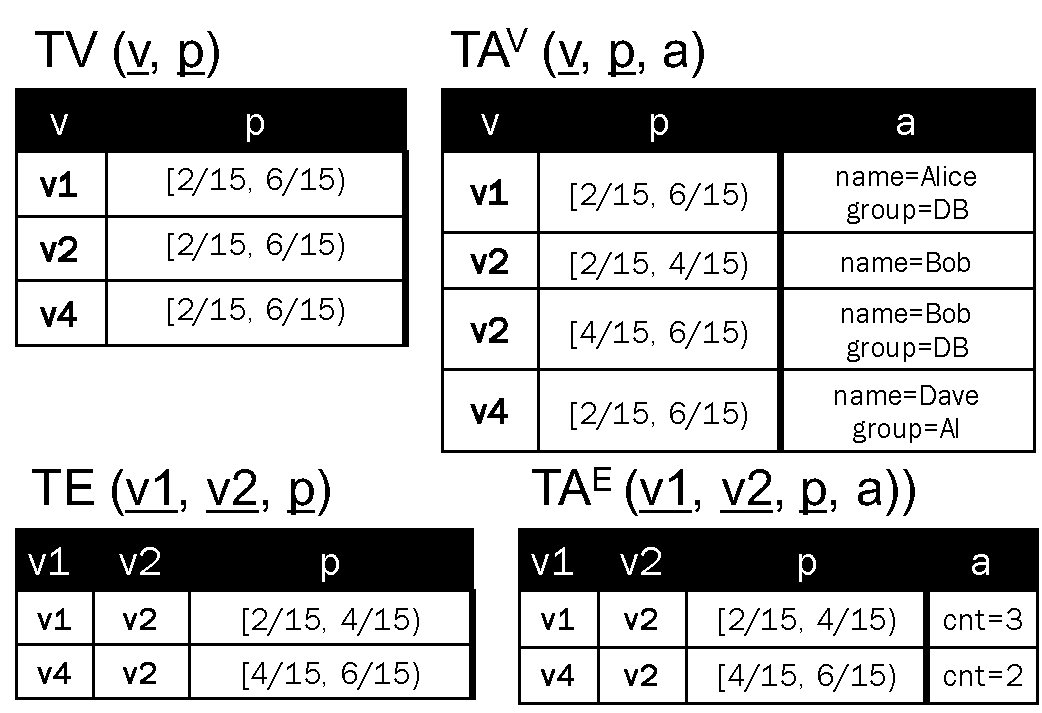
\includegraphics[width=2.5in]{figs/T2_rel.pdf}
\vspace{-0.5cm}
\caption{T2.}
\vspace{-0.5cm}
\label{fig:tg_t2}
\end{minipage}
\begin{minipage}[b]{4.3in}
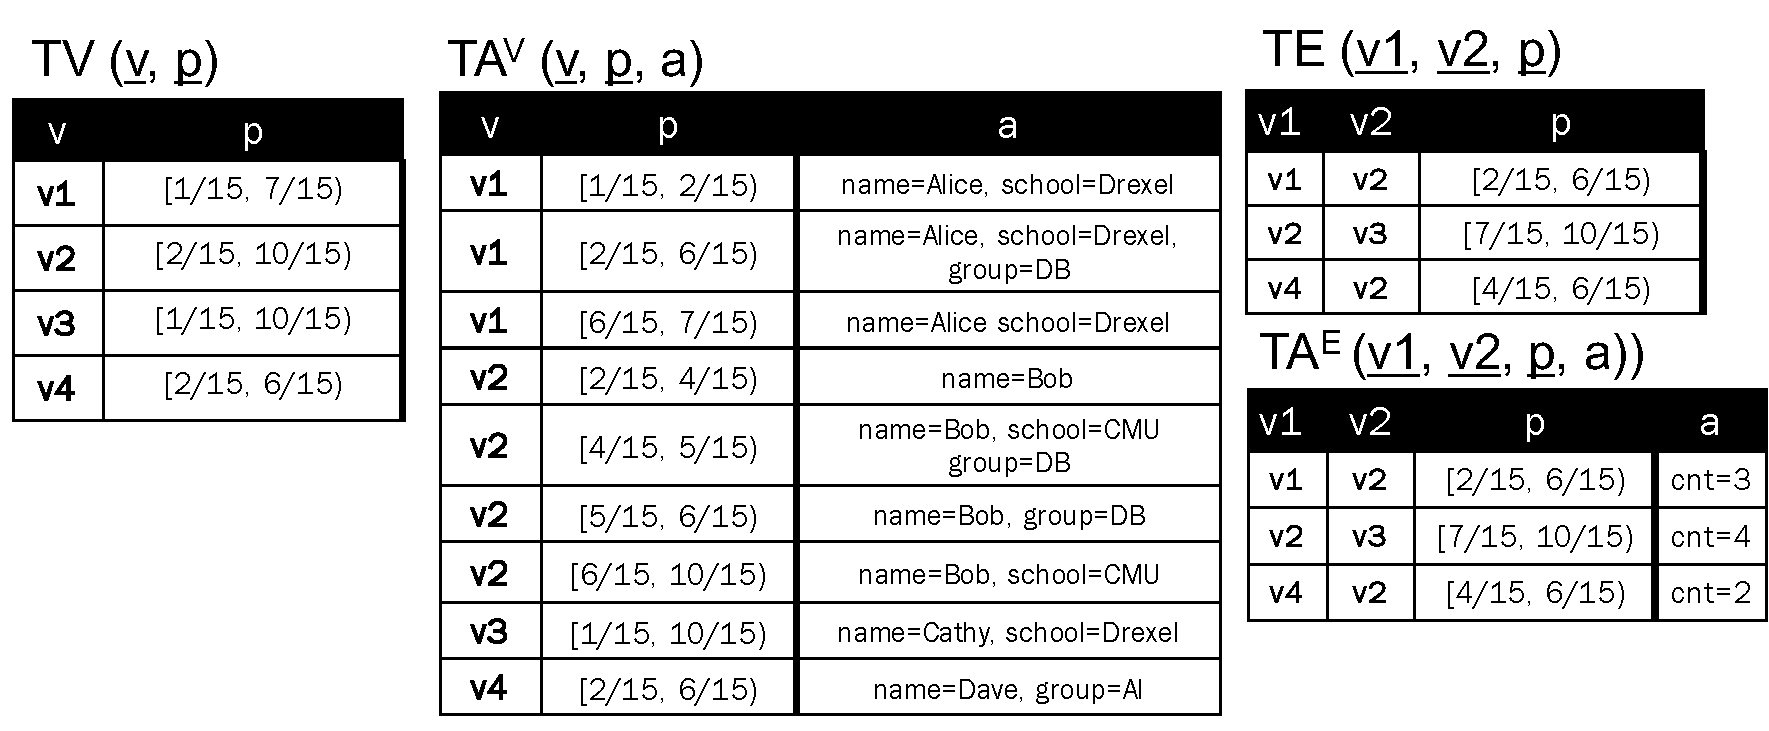
\includegraphics[width=4.3in]{figs/T1_union_T2_rel.pdf}
\vspace{-0.5cm}
\caption{$T1 \cup^T T2.$}
\label{fig:tg_union}
\vspace{-0.5cm}
\end{minipage}
%\caption{Binary operators.}
%\label{fig:binary}
\end{figure*}

We support temporal versions of the three binary set operators
intersection ($\cap^T$), union ($\cup^T$), and difference
($\setminus^T$).

\eat{These \tra operators are not schema robust~\cite{Dignos2012} ---
  their result is affected if the argument relation is extended by an
  additional attribute.  This presents a problem when executing the
  set operations over the \tav and \tae relations as there is no
  guarantee that a vertex or an edge with the same identity and at the
  same time instant has the same attribute set.  Thus all three
  operators require that the resolve primitive be invoked as part of
  the computation.}

To compute $\insql{T1} \cup^T \insql{T2}$, we set $\tv' = \tv_1 \cup^T
\tv_2$ and $\te' = \te_1 \cup^T \te_2$.  Next, we compute $\tav' =
\resolve{f_v}{\tav_1 \fullouterjoin^T_{v} \tav_2}$ and $\tae' =
\resolve{f_e}{\tae_1 \fullouterjoin^T_{v1,v2} \tae_2}$. 

Consider \insql{T1} in Figure~\ref{fig:tg_ve} and \insql{T2} in
Figure~\ref{fig:tg_t2}.  Figure~\ref{fig:tg_union} illustrates
\insql{T1} $\cup^T$ \insql{T2}.  According to the definition of
$\cup^T$, periods are split to coincide for any group, and thus the
attribute values for e.g., $v_1$ have three distinct tuples.

To compute $\insql{T1} \cap^T \insql{T2}$, we set $\tv' = \tv_1 \cap^T
\tv_2$ and $\te' = \te_1 \cap^T \te_2$.  Next, we compute $\tav' =
\constr{\resolve{f_v}{\tav_1 \fullouterjoin^T_{v} \tav_2}}{\tv'}$ and
$\tae' = \constr{\resolve{f_e}{\tae_1 \fullouterjoin^T_{v1,v2}
    \tae_2}}{\te'}$.

As an example, when applying \insql{T1} $\cap^T$ \insql{T2}, only the
vertices and edges present in both \tgs are produced, thus eliminating
$v_3$ and $v_4$.  Period $[2/15, 4/15)$ for $v_2$ is computed as a
  result of the join of $[2/15, 5/15)$ in \insql{T1} and [$2/15,
      4/15)$ in \insql{T2}.  See Figure~\ref{fig:tg_inter} in
      Appendix~\ref{sec:app:examples} for full result.

To compute $\insql{T1} \setminus^T \insql{T2}$, we set $\tv' = \tv_1
\setminus^T \tv_2$ and $\te' = \te_1 \setminus^T \te_2$.  Next, we
compute $\tav' = \constr{{\tav}'_1}{\tv'}$ and $\tae' =
\constr{{\tae}'_1}{\te'}$.

To continue the example above, the result of \insql{T1} $\setminus^T$
\insql{T2} includes vertex v1 before 2/15 and after 6/15, splitting
one v1 tuple in \tv of T1 into two temporally-disjoint tuples in the
result.  See Figure~\ref{fig:tg_diff} in
Appendix~\ref{sec:app:examples} for full result.

Note that both $\cap^T$ and $\cup^T$ require that resolve be invoked,
to reconcile the vertex/edge attributes associated with vertices/edges
in the temporal intersection of the inputs.

\eat{Note also that $\tav'$ and $\tae'$ are constrained w.r.t. $\tv'$ and
$\te'$, respectively, in the expressions above.}

 \eat{Then $\tve_1 \oplus_{f_v,f_e} \tve_2 = \{ \tv_1 \oplus \tv_2,
   \te_1 \oplus \te_2, \pi^T_{v,red(a_1,a_2)}(\tav_1
   \fullouterjoin^T_{v}
   \tav_2),$\\ $\pi^T_{v_1,v_2,red(a_1,a_2)}(\tae_1
   \fullouterjoin^T_{v_1,v_2} \tae_2) \}$, with all FK constraints on
   \tav and \tae enforced.}

\eat{As elsewhere, the default reduce function is \insql{set}.  In addition
to the functions defined in Section~\ref{sec:algebra:agg} we also
support \{ \insql{left} | \insql{right} \}, which select the attribute
of the left, resp. right, operand.}

%\subsection{Temporal graph intersection}
%\label{sec:algebra:join}
\eat{
The binary temporal graph intersection operation $\trga \cap \trgb$
computes a temporal join~\cite{Gao2005} of \trga and \trgb with the
predicate $\trga.p \cap \trgb.p \neq \emptyset$, producing a tuple for
each pair of representative graphs for which time periods intersect:
$\trga \cap \trgb = \{(g_1 \cap g_2, p_1 \cap p_2)~|~((g_1, p_1) \in
\trga \wedge (g_2, p_2) \in \trgb \wedge p_1 \cap p_2 \neq \emptyset
\}$.  The result of $g_1 \cap g_2$ is computed by intersecting the
sets of vertices and of edges of the graphs~\cite{GraphTheory}.  For
each vertex and edge in the result, we compute a {\em union} of their
bags of properties.% \julia{Figure with example.}
%
Algorithm~\ref{alg:inter} presents the evaluation of $\tvea \cap
\tveb$. We compute temporal joins over \tv and \te (lines 1, 2).  We
then compute \tav' and \tae' with temporal outer joins of the
corresponding relations (lines 3, 4).  Finally, we enforce foreign key
constraints on \te', \tav' and \tae' (lines 5, 6).
}

\eat{In addition to invoking reduce on the attribute relations for all
operations, it is required to invoke $\constr{\tav'}{\tv}$ and
$\constr{\tae'}{\te}$ for }

\eat{{\bf R1, R2}: for all set operators coalesce every relation in
$\ttt'$; {\bf R3}: enforce FK on $\tav'$ and $\tae'$ for difference,
intersection. {\bf R4}: require reduce function.}

\eat{Intersection and union may uncoalesce, while difference does not.
  Intersection and difference require FK enforcement for \tav and
  \tae, while union does not.}

%\subsection{Temporal graph union}
%\label{sec:algebra:outerjoin}

\eat{
The binary temporal graph union operation $\trga \cup \trgb$ computes
a temporal full outer join~\cite{Gao2005} of \trga and \trgb on the
predicate $\trga.p \cap \trgb.p $. For tuples $(g_1, p_1) \in \trga$
and $(g_2, p_2) \in \trgb$ for which $p_1 \cap p_2 \neq \emptyset$, we
compute $(g_1 \cup g_2, p_1 \cap p_2)$.  The result of $g_1 \cup g_2$
is computed by taking a {\em union} of the sets of vertices and of
edges of the graphs~\cite{GraphTheory}.  For each vertex and edge in
the result, we compute a {\em union} of their bags of properties.
Tuples from \trga (resp. \trgb) for which there does not exist a tuple
in \trgb (resp. \trga) for part or all of the validity period are
included in the result of the full outer join. 
}

\eat{
 $\trg_1 \cup \trg_2 = \{ (g, p) | (g_1, p_1) \in \trg_1 \wedge (g_2,
p_2) \in \trg_2 \wedge ((g = g_1 \cup g_2 \wedge p = p_1 \cap p_2
\wedge p_1 \cap p_2 \neq \emptyset) \vee (g = g_1 \wedge p = p_1 - p_2
\wedge \nexists p \in \trg_2 = p_1 - p_2) \vee (g = g_2 \wedge p = p_2
- p_1 \wedge \nexists p \in \trg_1 = p_2 - p_1))\}$.  Similar to
temporal intersection, temporal union is essentially an outer
theta-join of $\trg_1$ and $\trg_2$ with a $p_1 \cap p_2$ predicate.
We use the standard graph union definition based on set theory, which
computes unions of the vertex and edge sets from the two
operands~\cite{GraphTheory}.}

\eat{
Algorithm~\ref{alg:union} presents the evaluation of $\tvea \cup
\tveb$.  We compute temporal outer joins over the corresponding \tv,
\te, \tav and \tae.
}

\eat{\begin{algorithm}[t]
\caption{Temporal graph union in \tve.}
\begin{algorithmic}[1]
\REQUIRE $\tvea, \tveb$.\\
\STATE $\tv' = \tv_1 \fullouterjoin^T_v \tv_2$\\
\STATE $\te' = \te_1 \fullouterjoin^T_{v1,v2} \te_2$\\
\STATE $\tav' = \cl (\pi_{v,p,\tav_1.a \cup \tav_2.a}\tav_1 \fullouterjoin^T_v \tav_2)$\\
\STATE $\tae' = \cl (\pi_{v_1,v_2,p,\tae_1.a \cup \tae_2.a}\tae_1 \fullouterjoin^T_{v1,v2} \tae_2)$\\
\RETURN new $\tve (\tv';\te';\tav';\tae')$\\
\end{algorithmic}
\label{alg:union}
\end{algorithm}
}

%\subsection{Temporal graph difference}
%\label{sec:algebra:diff}

\eat{
The binary temporal graph difference operation $\trga \setminus \trgb$
computes a temporal left outer join~\cite{Gao2005} of \trga and \trgb
on the predicate $\trga.p \cap \trgb.p$.  For tuples $(g_1, p_1) \in
\trga$ and $(g_2, p_2) \in \trgb$ for which $p_1 \cap p2 \neq
\emptyset$, we compute $(g_1 \setminus g_2, p_1 \cap p_2)$.  The
result of $g_1 \setminus g_2$ is computed by taking a {\em set
  difference} of the sets of vertices and of edges of the graphs.  For
each vertex and edge in the result, we compute a {\em union} of their
bags of properties.  Tuples in \trga for which there does not exist a
tuple in \trgb for part or all of the validity period are included in
the result of the left outer join.
}
\eat{
Algorithm~\ref{alg:diff} presents the evaluation of $\tvea \setminus
\tveb$.  We compute temporal left outer joins over the corresponding
\tv and \te (lines 1,2).  We then compute $\tav'$ and $\tae'$ with
temporal outer joins of the corresponding relations (lines 3, 4).
Finally, we enforce foreign key constraints on $\te'$, $\tav'$, and
$\tae'$ (lines 5, 6).
}

\eat{\begin{algorithm}[b]
\caption{Temporal graph difference in \tve.}
\begin{algorithmic}[1]
\REQUIRE $\tvea, \tveb$.\\
\STATE $\tv' = \tv_1 \leftouterjoin^T_v \tv_2$\\ 
\STATE $\te' = \te_1 \leftouterjoin^T_{v_1,v_2} \te_2$\\ 
\STATE $\tav' = \cl (\pi_{v,p,\tav_1.a \cup \tav_2.a}\tav_1 \fullouterjoin^T_v \tav_2)$\\
\STATE $\tae' = \cl (\pi_{v_1,v_2,p,\tae_1.a \cup \tae_2.a}\tae_1 \fullouterjoin^T_{v_1,v_2} \tae_2)$\\
\STATE enforce foreign keys on $\tav'$ w.r.t. $\tv'$\\ 
\STATE enforce foreign keys on $\tae'$ w.r.t. $\te'$\\ 
\RETURN new $\tve (\tv';\te';\tav';\tae')$\\
\end{algorithmic}
\label{alg:diff}
\end{algorithm}
}

\subsection{Node creation}
\label{sec:algebra:ncreate}

\begin{figure}[b]
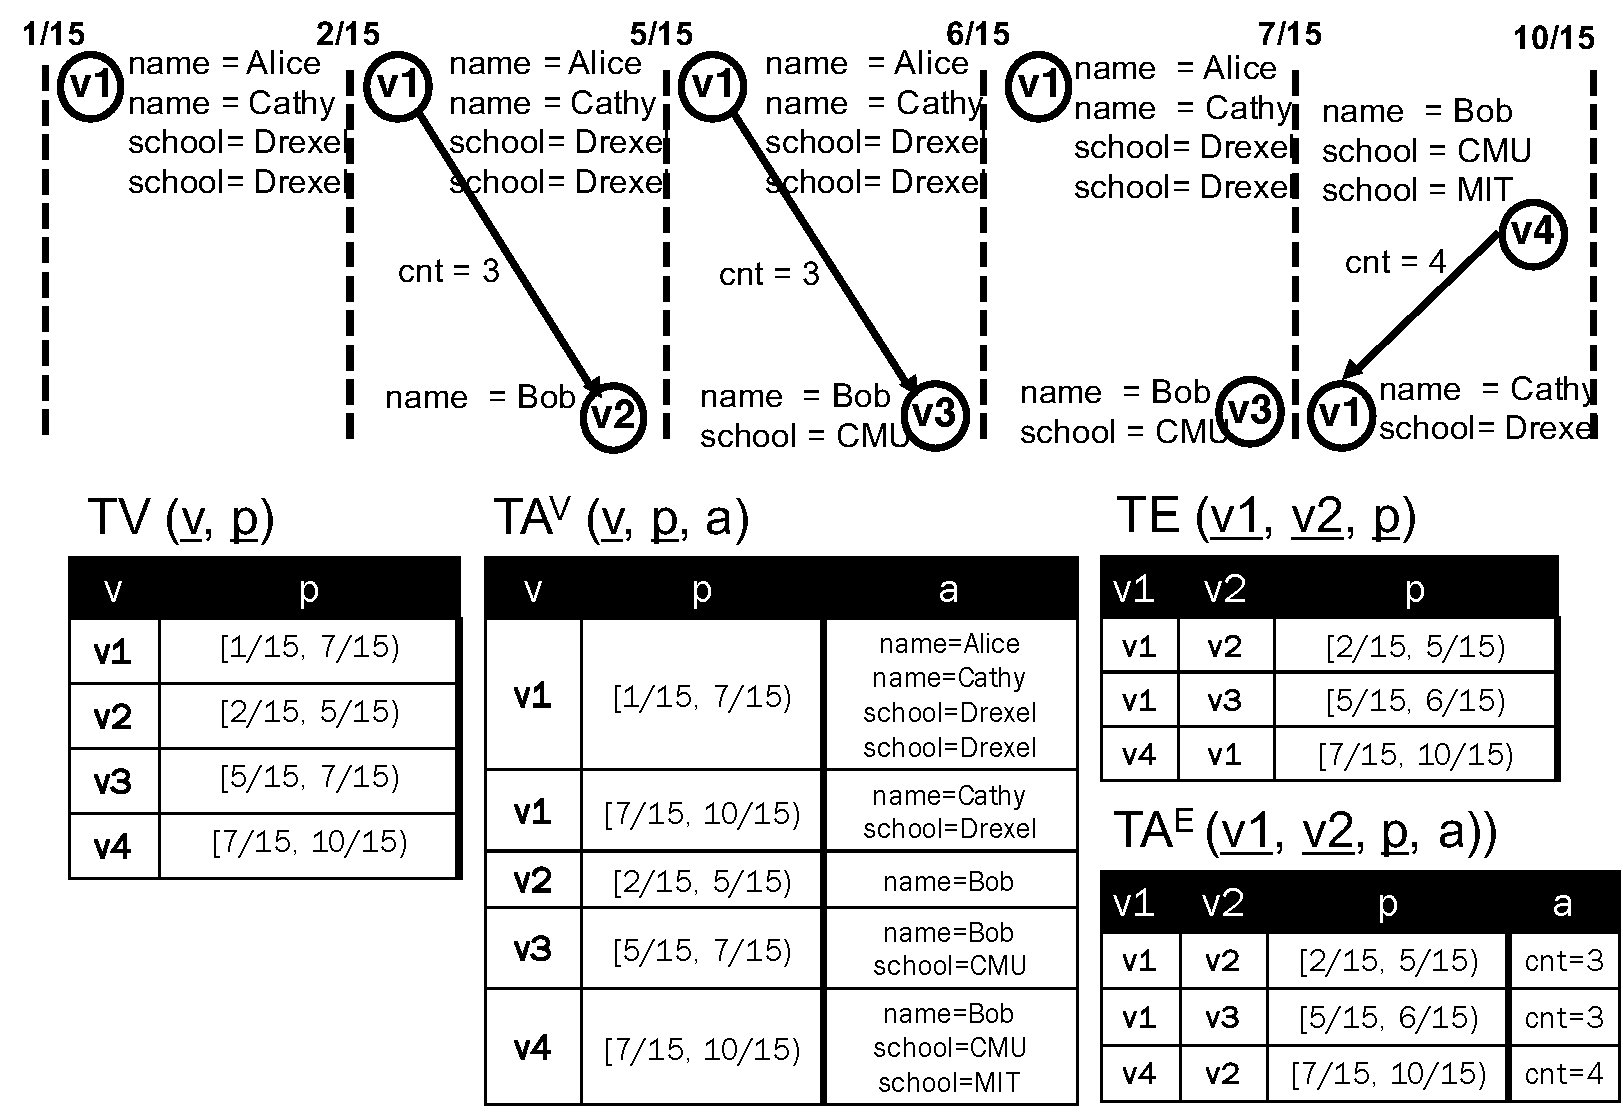
\includegraphics[width=3in]{figs/agg3.pdf}
\vspace{-0.2cm}
\caption{\insql{node}$^T_a(school, set(school), max(cnt).)$}
\vspace{-0.4cm}
\label{fig:tg_agg3}
\end{figure}

The node creation operator enables the user to analyze an evolving
graph at different levels of granularity.  This operator comes in two
variants --- based on vertex attributes or based on temporal window.

{\bf Attribute-based node creation} is denoted\\
$\insql{node}^T_a(g_1,\ldots,g_i,f_{v1}(k_1),\ldots,f_{vn}(k_n),f_{e1}(l_1),\ldots,f_{em}(l_m),\tve)$,
where $g_1,\ldots,g_i$ are the grouping attributes, and each
$f_{vj}(k_j)$ ($f_{ej}(l_j)$) specifies an aggregation function
$f_{vj}$ (resp. $f_{ej}$) to be applied to a vertex property $k_j$
(resp. edge property $l_j$).  This operation allows the user to
generate a \tg in which vertices correspond to disjoint groups of
vertices in the input that agree on the values of all grouping
attributes.  For example, $\insql{node}^T_a(school,\tve)$ will compute
a vertex for each value of $\tav.a.school$.  Vertices that do not
specify a value for one or several grouping attributes at a given
time, will not contribute to the result for the corresponding
snapshot.

To compute $\tve' =
\insql{node}^T_a(g_1,\ldots,g_i,f_{v1}(k_1),\ldots,f_{vn}(k_n),$
\\ $f_{e1}(l_1),\ldots,f_{em}(l_m),\tve)$, we execute $L =
g_1,\ldots,g_i \gamma^T (\tv \rightouterjoin^T_v \tav)$, computing an
intermediate temporal relation for each group.  Next, we generate the
new vertex relation $\tv'$, by generating an id for each group with a
Skolem function: $\tv' = \sigma^T_{skolem(g_1,\ldots,g_i)}L$.

Then, $\tav' = \resolve{f_{v1}(k_1), \ldots,
  f_{vn}(k_n)}{\sigma^T_{skolem(g_1,\ldots,g_i), a} L}$.  Note the use
of the resolve primitive to reconcile attribute values within a group.

Vertices of the input are partitioned on their values of the grouping
attributes.  Partitioning of the vertices also induces a partitioning
of the edges. To compute the new edges $\te'$, we generate a temporal
conjunctive query that computes $E(v_1,v_2,p,v_1',v_2')$, where $v_1'$
and $v_2'$ are the identifiers of the vertices in \tv' to which $v_1$
and $v_2$ are mapped.  Finally, we compute $\te' =
\coal{\pi_{v_1',v_2',p}E}$ and\\ $\tae' =
\resolve{f_{e1}(l_1),\ldots,f_{vm}(l_m)}{v_1',v_2' \gamma^T (E
  \bowtie^T_{v_1,v_2} \tae)}$.

Figure~\ref{fig:tg_agg3} illustrates attribute-based node creation
over \insql{T1} in our running example, with \insql{set(school)}
aggregation function for vertices and and \insql{max(cnt)} for edges.
Vertices $v_1$ and $v_3$ create a single new vertex $v_10$,
representing Drexel.

{\bf Window-based node creation} is denoted\\
$\insql{node}^T_w(w,q_v,q_e,f_{v1}(k_1),\ldots,f_{vn}(k_n),f_{e1}(l_1),\ldots,f_{em}(l_m),\tve)$,
where $w$ is the window specification, $q_v$ and $q_e$ are vertex and
edge quantifiers, and each $f_{vj}(k_j)$ ($f_{ej}(l_j)$) specifies an
aggregation function $f_{vj}$ (resp. $f_{ej}$) to be applied to a
vertex property $k_j$ (resp. edge property $l_j$).  This operation
corresponds to moving window temporal aggregation, and is inspired by
the stream aggregation work of~\cite{Li2005} and by generalized
quantifiers of~\cite{Hsu1995}, both adopted to graphs.

\eat{We argued in the introduction that it is interesting and
  insightful to analyze an evolving graph at different levels of
  granularity.  For example, the user may want to aggregate multiple
  consecutive representative graphs into a single representative
  graph, coarsening the granularity, or to predefine temporal
  resolution and look at the graph at that scale, irrespective of
  whether this resolution happens to be finer or coarse than the
  natural evolution rate of the graph.  For this, we introduce a node
  creation operator which is similar to the {\em moving window
    temporal aggregation} in temporal relational algebra.  Our
  approach is inspired by stream aggregation work of~\cite{Li2005},
  adopted to graphs, and by generalized quantifiers
  of~\cite{Hsu1995}.}

\eat{Node creation is denoted $\ncr{G_V}{W,Q_V,Q_E,red}{\ttt}$,\\ where
$G_V$ are the grouping attributes, $W$ is the window specification,
$Q_V$ and $Q_E$ are vertex and edge quantifiers, and $red$ is the set
of reduce functions.  It produces a consolidated evolving graph with
specific temporal granularity.}

\eat{{\em Grouping attributes} $G_V$ are vertex properties by which
vertices are grouped into new entities, similar to \insql{GROUP BY}
clause in SQL.  Since node creation requires new identifiers, the
combination of the grouping properties can be used in a mechanism
equivalent to a Skolem function.  The simplest, default grouping
attribute is the $vid$ of the vertex.}

Window specification $w$ is of the form $n~\{unit|\insql{changes}\}$,
where $n$ is an integer, and $unit$ is a time unit, e.g., $10~min$,
$3~years$, or any multiple of the usual time units.  When $w$ is the
form $n~\insql{changes}$, it defines the window by the number of
changes that occurred in \tve (affecting any of its constituent
relations). Window boundaries are computed left-to-right, i.e., from
least to most recent.  

\eat{Our window specification by change is similar to slide-by-row window
in stream aggregation~\cite{Li2005}.  Note that, because \tg algebra
is compositional, we do not support node creation with overlapping
windows, because it does not produce a valid \tg.  To see why this is
so, consider applying a sliding window of 3 months range with 1 month
slide to graph \insql{T} in Figure~\ref{fig:tg_ve}.  We would produce
the following tuples for $v_1$: $(v_1, [1/15, 4/15), a_1)$, $(v_1,
  [2/15, 5/15), a_2)$, $(v_1, [3/15, 6/15))$, and so on, which clearly
      violates the temporally coalesced requirement in
      definition~\ref{tg}.}

\eat{Similar to~\cite{Li2005} we support creation simultaneously by
  time and by non-temporal attributes (e.g., vertex properties).  If
  the window specification is one change, then the operation devolves
  into pure structural reduce or node creation, as classified by
  Wood~\cite{Wood2012}.  If the grouping attribute is the vertex
  $vid$, then the operation is purely temporal, with no structural
  aspect.}

Vertex and edge quantifiers $q_v$ and $q_e$ are of the form \{
\insql{all} | \insql{most} | \insql{at least} $n$ | \insql{exists} \},
where $n$ is a decimal representing the percentage of the time during
which a vertex or an edge existed, relative to the duration of the
window (\insql{exists} is the default).  Quantifiers are useful for
observing different kinds of temporal evolution, e.g., to observe only
strong connections over a volatile evolving graph, we may want to only
include vertices that span the entire window ($q_v=\insql{all}$), and
edges that span a large portion of the window ($q_e=\insql{most}$).
 
\eat{The optional reduce functions compute new values for vertex and
  edge properties representative of the whole window, e.g.,
  $any(name), last(school), sum(cnt)$.}
%
 
\eat{Key-value pairs for vertex and edge properties for which no
aggregation functions are specified, are collected into a bag
corresponding to the entity in the result.  These can be subsequently
transformed with $map^T$ (Section~\ref{sec:algebra:project}).}

\eat{ 
Temporal aggregation over \tve follows the outline of
Algorithm~\ref{alg:op}, but requires an additional step, and is
revisited in Algorithm~\ref{alg:agg_ve}.
%
}

For both kinds of window specification (by unit or by number of
changes), we must (1) compute a mapping from a tuple in a temporal
relation to one or multiple windows, and (2) aggregate over each
window.  The $s$ parameter for the split primitive is the smallest
start date across \tve.

To compute $\tv'$, we apply split to \tv, group by vid, select only
those vertices that meet the quantification, and finally coalesce:
$\tv' = \coal{\sigma^T_{q_V} (v \gamma^T_{\cup
    p}(\wsplit{s}{w}{\tv}))}$.  Similarly for $\te'$.  To compute
attribute relations we split, resolve with the aggregation functions,
and constrain: $\tav' =
\constr{\resolve{f_{v1}(k_1),\ldots,f_{vn}(k_n)}{\wsplit{s}{w}{\tav}}}{\tv'}$,
similarly for $\tae'$.

\eat{We compute group periods based on window
specification: $P = \textsf{computePeriods}(W, \tv, \te, \tav, \tae)$.
We use temporal aggregation and selection to evaluate $Q_V$ on each
group in $\tv$: $\tv' = \sigma_{P,Q_V}( _{G_V}\vartheta^T (\tv
\leftouterjoin^T \tav))$ and similarly for $\te$: $\te' =
\sigma_{P,Q_E}( _{G_V}\vartheta^T (\te \bowtie^T_{v_1=v} \tav
\bowtie^T_{v_2=v} \tav))$.  The edge triplets, obtained through
three-way temporal join of \tae with \tav are required to aggregate
edges by $G_V$.  }

\eat{
Node creation over \trg is computed by first calculating time periods
from $W$ and \trg, and then reducing and combining the representative
graphs directly.
}

\begin{figure*}[t]
%\centering
\begin{subfigure}[b]{0.5\textwidth}
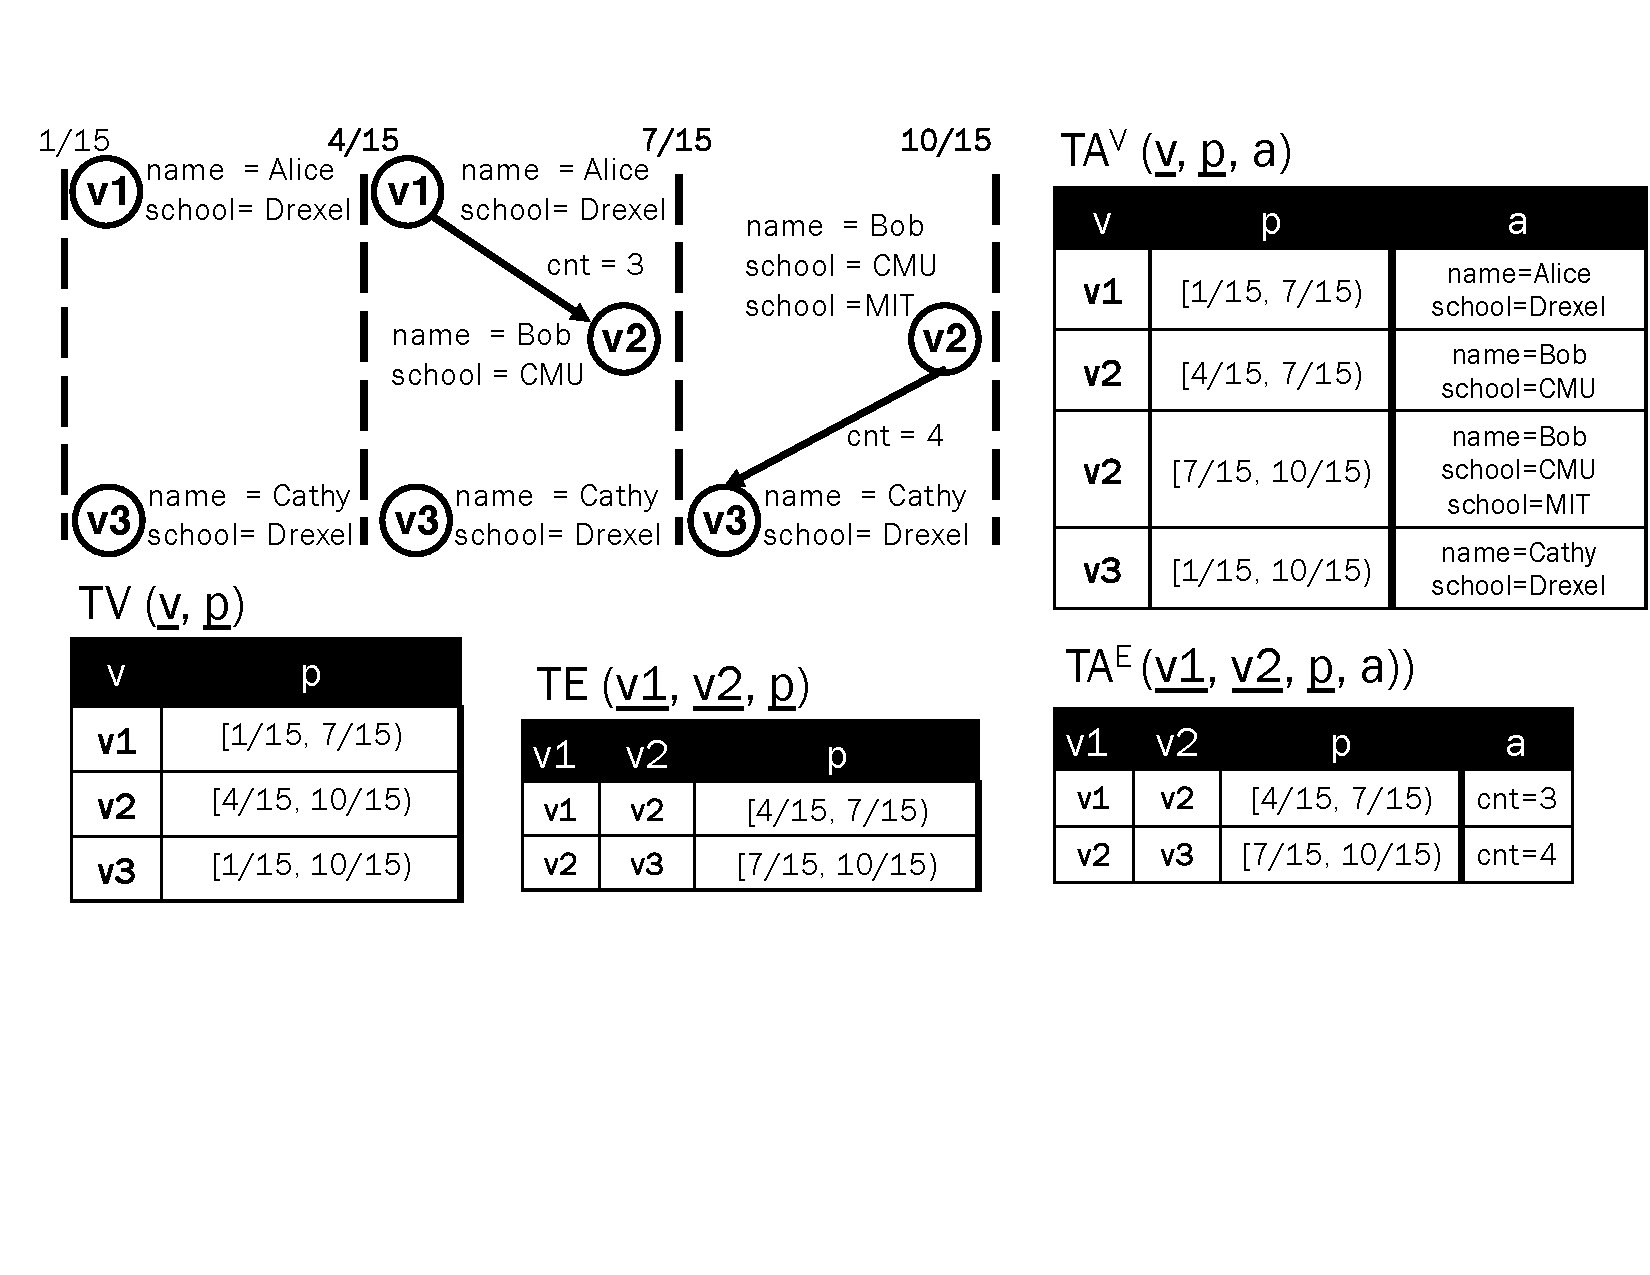
\includegraphics[width=3.2in]{figs/agg1.pdf}
\caption{By time: $w=3~\textsf{months}$.}
\label{fig:tg_agg1}
\vspace{-0.2cm}
\end{subfigure}
\begin{subfigure}[b]{0.5\textwidth}
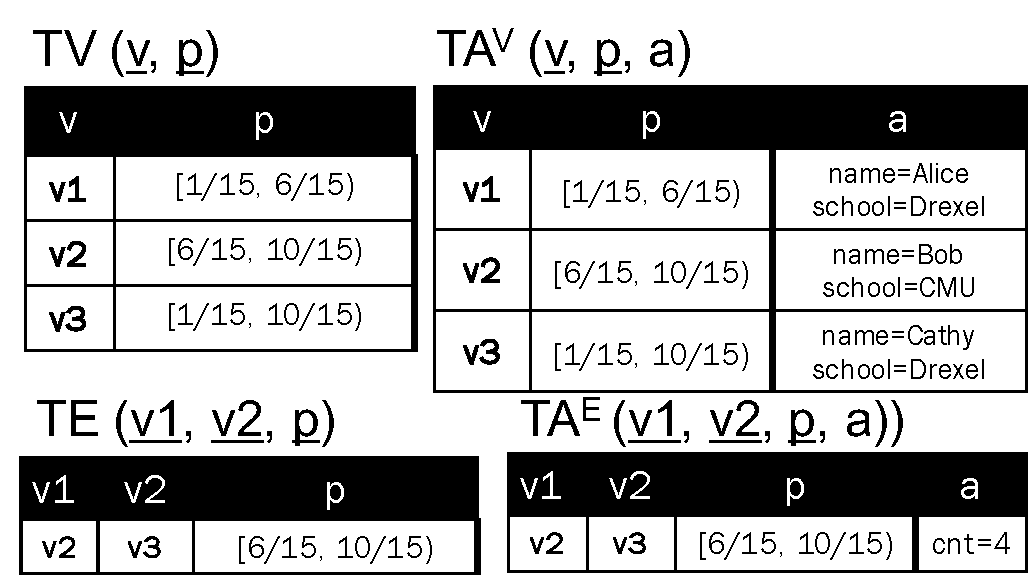
\includegraphics[width=3.2in]{figs/agg2.pdf}
\caption{By change: $w=3~\textsf{changes}$.}
\label{fig:tg_agg2}
\end{subfigure}
\caption[]{Node creation,
  $\insql{node}^T_w(\mathsf{q_v=always},\mathsf{q_e=exists,f_v=\{first(name),~first(school)\}},\ttt)$.}
\vspace{-0.2cm}
\label{fig:tg_agg}
\vspace{-0.2cm}
\end{figure*}

\eat{\begin{algorithm}[t!]
\caption{Node creation in \tve.}
\begin{algorithmic}[1]
\REQUIRE \tve (\tv;\te;\tav;\tae), window specification $W$, vertex
quantifier $Q_V$, edge quantifier $Q_E$, vertex aggregate function
$A_V$, vertex aggregate function $A_E$.\\
\STATE $P = \textsf{computePeriods}(W, \tv, \te, \tav, \tae)$\\
\STATE  $\tv' = \cl (_{G_V}\vartheta_{P,Q_V}(\tv))$\\
\STATE  $\te' = \cl (_{G_V}\vartheta_{P,Q_E}(\te))$\\
\STATE  $\tav' = \cl (_{G_V}\vartheta_{P,A_V}(\tav))$\\
\STATE  $\tae' = \cl (_{G_V}\vartheta_{P,A_E}(\tae))$\\
\STATE  follow steps 5-7 of Algorithm~\ref{alg:op}\\
%\STATE  enforce foreign keys on $\te'$ w.r.t. $\tv'$\\
%\STATE  enforce foreign keys on $\tav'$ w.r.t. $\tv'$\\
%\STATE  enforce foreign keys on $\tae'$ w.r.t. $\te'$\\
\RETURN new $\tve (\tv';\te';\tav';\tae')$\\
\end{algorithmic}
\label{alg:agg_ve}
\end{algorithm}
}

Figure~\ref{fig:tg_agg1} illustrates window-based node creation by
time ($w=3~\textsf{months}$), and Figure~\ref{fig:tg_agg2} --- by
change ($w=3~\textsf{changes}$).  Both are applied to \insql{T1} in
our running example with \insql{all} quantifier for vertices and
\insql{exists} for edges, and \insql{first} aggregation function for
vertex and edge properties.  $v_2$ is present in the result in
Figure~\ref{fig:tg_agg1} starting at $4/15$ because it did not exist
for the entirety of the first window, while in
Figure~\ref{fig:tg_agg2} it is produced starting $6/15$.

\eat{Node creation may uncoalesce and requires FK enforcement.}

\eat{{\bf R1, R2}: coalesce every relation in $\ttt'$; {\bf R3}:
  enforce FK on $\tav', \te', \tae'$; {\bf R4}: require reduce
  function.}

\eat{ Our aggregation quantifiers are inspired by generalized
  quantifiers of~\cite{Hsu1995} with n-place delimiters.  $Q(R)$ as a
  Boolean-valued function of a relation''~\cite{Hsu1995}.  A
  quantifier contains an n-place determiner, e.g., ``at least one
  vertex in each window for each group'' is a 2-place determiner
  quantifier.  \tg algebra supports determiners from the set
  $\{at\ least\ one, all, most, at\ least\ n\}$, where $n$ is an
  integer representing a ratio.  $all$ is a usual universal quantifier
  that in standard SQL can be achieved with the use of two \insql{NOT
    EXISTS}.}

\subsection{Edge creation}
\label{sec:algebra:ecreate}

Edge creation
$\insql{edge}^T(q,f_1(k_1),\ldots,f_n(k_n),\ttt_1,\ttt_2)$ is a binary
operator that computes a \tg on the vertices $\tv = \tv_1 \cup^T
\tv_2$, with edges and edge attributes computed by a conjunctive query
over the constituent relations of $\ttt_1$ and $\ttt_2$.  \eat{We compute}
$L(v_1,v_2,a,p) = \resolve{f_1(k_1),\ldots,f_n(k_n)}{q(\ttt_1,
  \ttt_2)}$, and then set $\te' = \coal{\pi^T_{v1,v2} L}$, and $\tae'
= \sigma_{a~is~not~null} L$.  We then compute $\tav =
\resolve{f_1(k_1),\ldots,f_n(k_n)}{\tv_1 \cup^T \tv_2}$.

\eat{$\ecr{\ttt_1}{q,red}{\ttt_2}$ be an edge creation operator, where $q$
is a conjunctive query over constituent relations of $\tve_1$ and
$\tve_2$ and $red$ is a reduce function. $q$ must return a valid
temporal relation $(v_1, v_2, a_1, a_2)$.  The reduce function is used
to compute the final $\tae'$ relation.  $\ecr{\ttt_1}{q,red}{\ttt_2} =
\{ \tv', \te', \tav', \tae' \}$, where $\tae' =
\sigma^T_{v_1,v_2,red(a_1,a_2)}(q(\ttt_1, \ttt_2))$ subject to FK
constraint from $\tv_1 \cup^T \tv_2$, $\te' =
\sigma^T_{v_1,v_2}(\tae')$, \tv' is a subset of $\tv_1 \cup^T \tv_2$
such that it contains only vertices with edges in $\te'$, and $\tav'$
is an empty relation.  Intuitively, edge creation returns a new \tg
from nodes of $\ttt_1$ and $\ttt_2$ with no attributes, connected by
edges determined by $q$.}

Edge creation has several important applications.  It can be used to
compute friend-of-friend edges (passing in the same \tg as both
arguments).  Since $q$ can include predicates over the timestamps,
$\insql{edge}^T$ can compute journeys.  A journey is a path in the
evolving graph with non-decreasing time
edges~\cite{Casteigts2011,Ferreira2004}.  By adding a temporal
condition to $q$, we can obtain journeys similar to time-concurrent
paths.

In graph theory, a graph join of two undirected unlabeled disjoint
graphs is defined as the union of the two graphs and additional edges
connecting every vertex in graph one with each vertex in graph two.
We can obtain a graph join by computing $\te' = \tv_1 \times^T \tv_2$.

SocialScope~\cite{Amer-Yahia2009} defines (non-temporal) graph
composition: compose the edge of the two operands and return an
edge-induced subgraph.  TGA can express this operator by a combination
of node creation and vertex subgraph.

\eat{In \ql temporal graph composition can be computed using node
  creation of \ttt with itself and a $q = $ a temporal theta-join of
  $\tae$ and $\tae_2$. }

%\julia{Example of edge transpose goes here.}

\eat{Note that edge creation produces new edges.  To add these edges to the
original graph, a subsequent union must be performed.}

\eat{Graph composition operator in our algebra is a temporal extension of
the composition operator in SocialScope~\cite{Amer-Yahia2009}.  It
produces a graph induced by edges that are composed from edges in the
two operands for any time point when they coexisted.  The value of the
new edge attributes is determined by the resolve function, similar to
the set based operators.}

\eat{
Let $\odot_{\delta,r}$ be a composition operator, where $\delta$ is a
directional condition pair $d_1=v_1|v_2, d_2=v_1|v_2$ and $r$ is a
resolve function.  Then $\ttt_1 \odot_{\delta,r} \ttt_2 = \{ \tv',
\te', \tav', \tae' \}$, where $\forall (v_x,v_z,p) \in \te' \exists
(d_1,v_x,p_1) \in \te_1 \wedge (d_2,v_z,p_2) \in \te_2 \wedge p=p_1
\cap p_2$, \tv' contains only vertices with edges in \te', with FK
constraint enforced on \tav' from \tv', and $\forall (v_x,v_z,p,a) \in
\tae' \exists (d_1,v_x,p_1,a_1) \in \tae_1 \wedge (d_2,v_z,p_2) \in
\tae_2 \wedge p=p_1 \cap p_2 \wedge a=r((a_1,p_1),(a_2,p_2))$.
}

\eat{{\bf R1, R2}: coalesce $\te'$ and $\tae'$; {\bf R3}: constraint $\te'$
on $\tv'$, $\tv'$ on $\te'$ (to remove nodes with no edges), and
$\tae'$ on $\te'$; {\bf R4}: require reduce function.}


\section{Analytics}
\label{sec:analytics}


%\section{Portal by Example}
\label{sec:example}

In this section we present \ql, a declarative query language for
evolving graphs. \ql uses SQL-like syntax, and has the form
\insql{TSelect} \ldots \insql{From} \ldots \insql{TWhere} \ldots
\insql{TGroup}.  We prefix temporal keywords with \insql{T}, to make
the distinction between \ql and SQL operations explicit.  We will use
\tgs \insql{T1} and \insql{T2} of Figures~\ref{fig:tg}
and~\ref{fig:tg_t2}, with structural schema V(\underline{vid}:int,
name:str, salary:int); E(\underline{vid1}:int, \underline{vid2}:int,
cnt:int), in our examples.

\subsection{Portal Basics}
\label{sec:example:basics}

{\bf Temporal selection.}  Consider query $Q1$ below.  

\begin{figure}
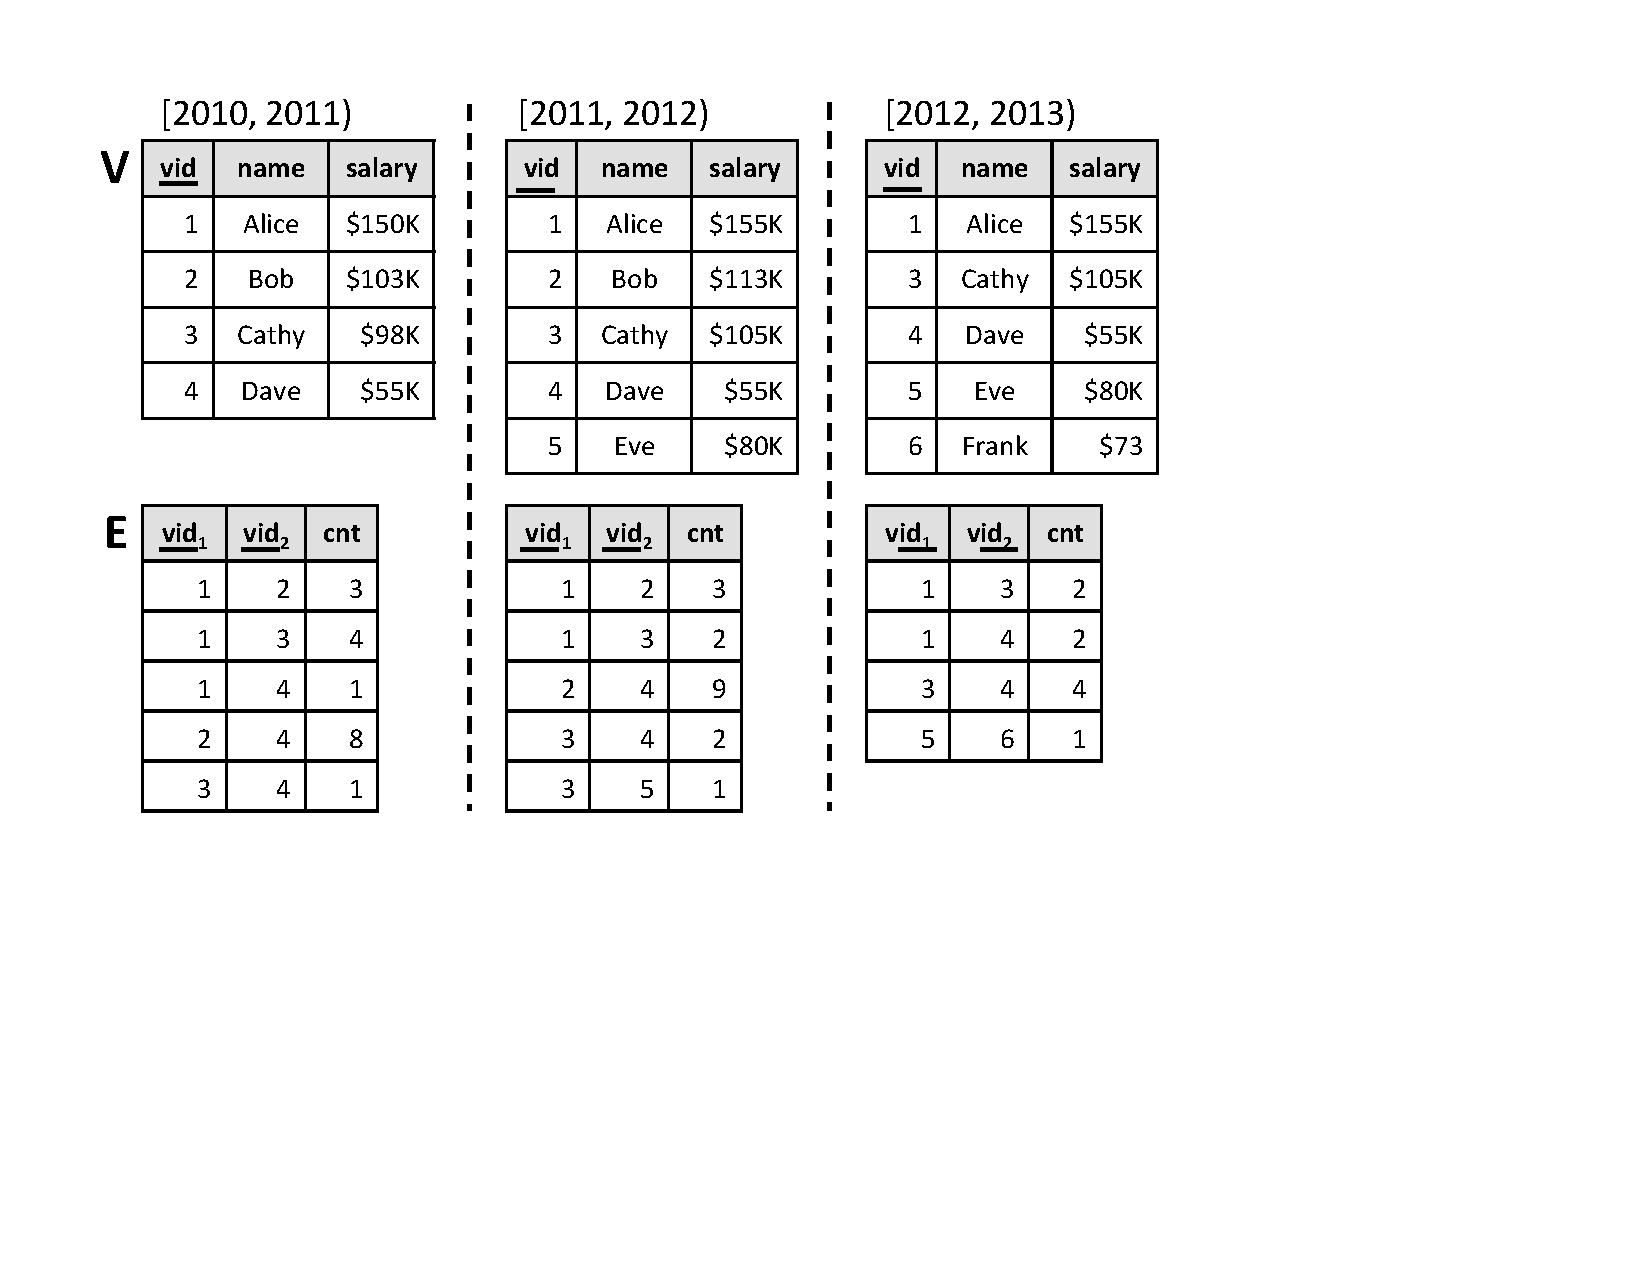
\includegraphics[width=3.5in]{figs/3VE.pdf}
\caption{Vertices and edges of 3 snapshots of \insql{T1}.}
\label{fig:3ve}
\end{figure}

\begin{small}
\begin{verbatim}
Q1: TSelect  V; E
    From     T1
    TWhere   Start >= 2010 And End < 2014
\end{verbatim}
\end{small}

$Q1$ performs temporal selection --- its result is a \tg that contains
a consecutive subset of the snapshots of \insql{T1} that fall within
the interval specified by the \insql{TWhere} clause, namely, $[2010,
  2011)$ through $[2013, 2014)$.  The result of $Q1$ has the same
    structural schema as \insql{T1}. The \insql{Start} or the
    \insql{End} portions of the \insql{TWhere} clause may be omitted.

More generally, the \insql{TWhere} clause supports a variety of
predicates based on which it is determined, for each snapshot in a
\tg, whether that snapshot is to be retained or discarded.  For
example, \insql{TWhere month(Start) like '\%r\%'} will retain all
snapshots that start during a month in which it is safe to eat oysters
(these are months with the letter 'r' in their name), while
\insql{TWhere year(End) \% 4 = 0} will retain snapshots that end in a
leap year, and discard all others.  However, recall from
Definition~\ref{def:tseq} that a temporal sequence, which constitutes
the temporal schema of a \tg, cannot have any gaps.  We enforce this
by never discarding a time interval in the middle of a sequence, but
rather replacing its snapshot with an empty graph $G(V=\emptyset;
E=\emptyset)$.

{\bf Specifying structural schema of the result.  Snapshot analytics.}
Next, consider query $Q2$ below.

\begin{small}
\begin{verbatim}
Q2: TSelect  V [vid, pagerank() as pr]; 
             E [vid1, vid2, cnt * 0.001 as score]
    From     T1
\end{verbatim}
\end{small}

This query illustrates how the \insql{TSelect} clause can be used to
specify the structural schema of the result, which in this case is
V(\underline{vid}:int, pr:float); E(\underline{vid1}:int,
\underline{vid2}:int, score:float).  We may use the \insql{TSelect}
clause to project out non-key columns of \insql{V} and \insql{E}, or
to add columns with computed values.  Data types of computed
attributes \insql{pr} and \insql{score} are determined by the return
type of the expressions that compute them.  Note that key columns of
\insql{V} and \insql{E} must be present in the result.

The value of the attribute \insql{pr} in $Q2$ is computed using a
snapshot analytic function \insql{pagerank()}.  \ql supports a variety
of snapshot analytics --- functions whose values are computed
w.r.t. each snapshot of a \tg --- including degree, shortest paths,
and connected components.  We provide an API that allows developers to
implement custom analytics that can either be computed locally at a
vertex, like degree, or be expressed in the popular Pregel
API~\cite{DBLP:conf/sigmod/MalewiczABDHLC10}.

\subsection{Temporal Aggregation and Join}
\label{sec:example:groupjoin}

{\bf Temporal aggregation} is illustrated by query $Q3$, which, when
executed with \insql{T1} from Figure~\ref{fig:tg} as input, computes
the \tg in Figure~\ref{fig:q3}.

\begin{small}
\begin{verbatim}
Q3: TSelect   Any V ; Any E 
    From      T1
    TGroup    by 2 years
\end{verbatim}
\end{small}

Temporal aggregation is a two-step operation.  First, temporal schema
of the output is computed according to Definition~\ref{def:tgroup}.
Then structural aggregation of Definition~\ref{def:sgroup} is used
over snapshots in the same temporal group.  Note the use of \insql{Any
  V} and \insql{Any E} in the \insql{TSelect} clause of $Q3$,
specifying that $\gamma^{V}$ and $\gamma^{E}$ operate over unions of
vertices and edges.  For an example consider snapshot $[2010, 2012)$
  in Figure~\ref{fig:q3}, which is computed from snapshots $[2010,
    2011)$ and $[2011, 2012)$ of \insql{T1} in Figure~\ref{fig:tg}.

We may use \insql{TGroup by Size} to specify that all snapshots of the
input \tg be aggregated into a 1-snapshot \tg.  This notation will be
useful when we discuss trend analytics later in this section.

\begin{figure}
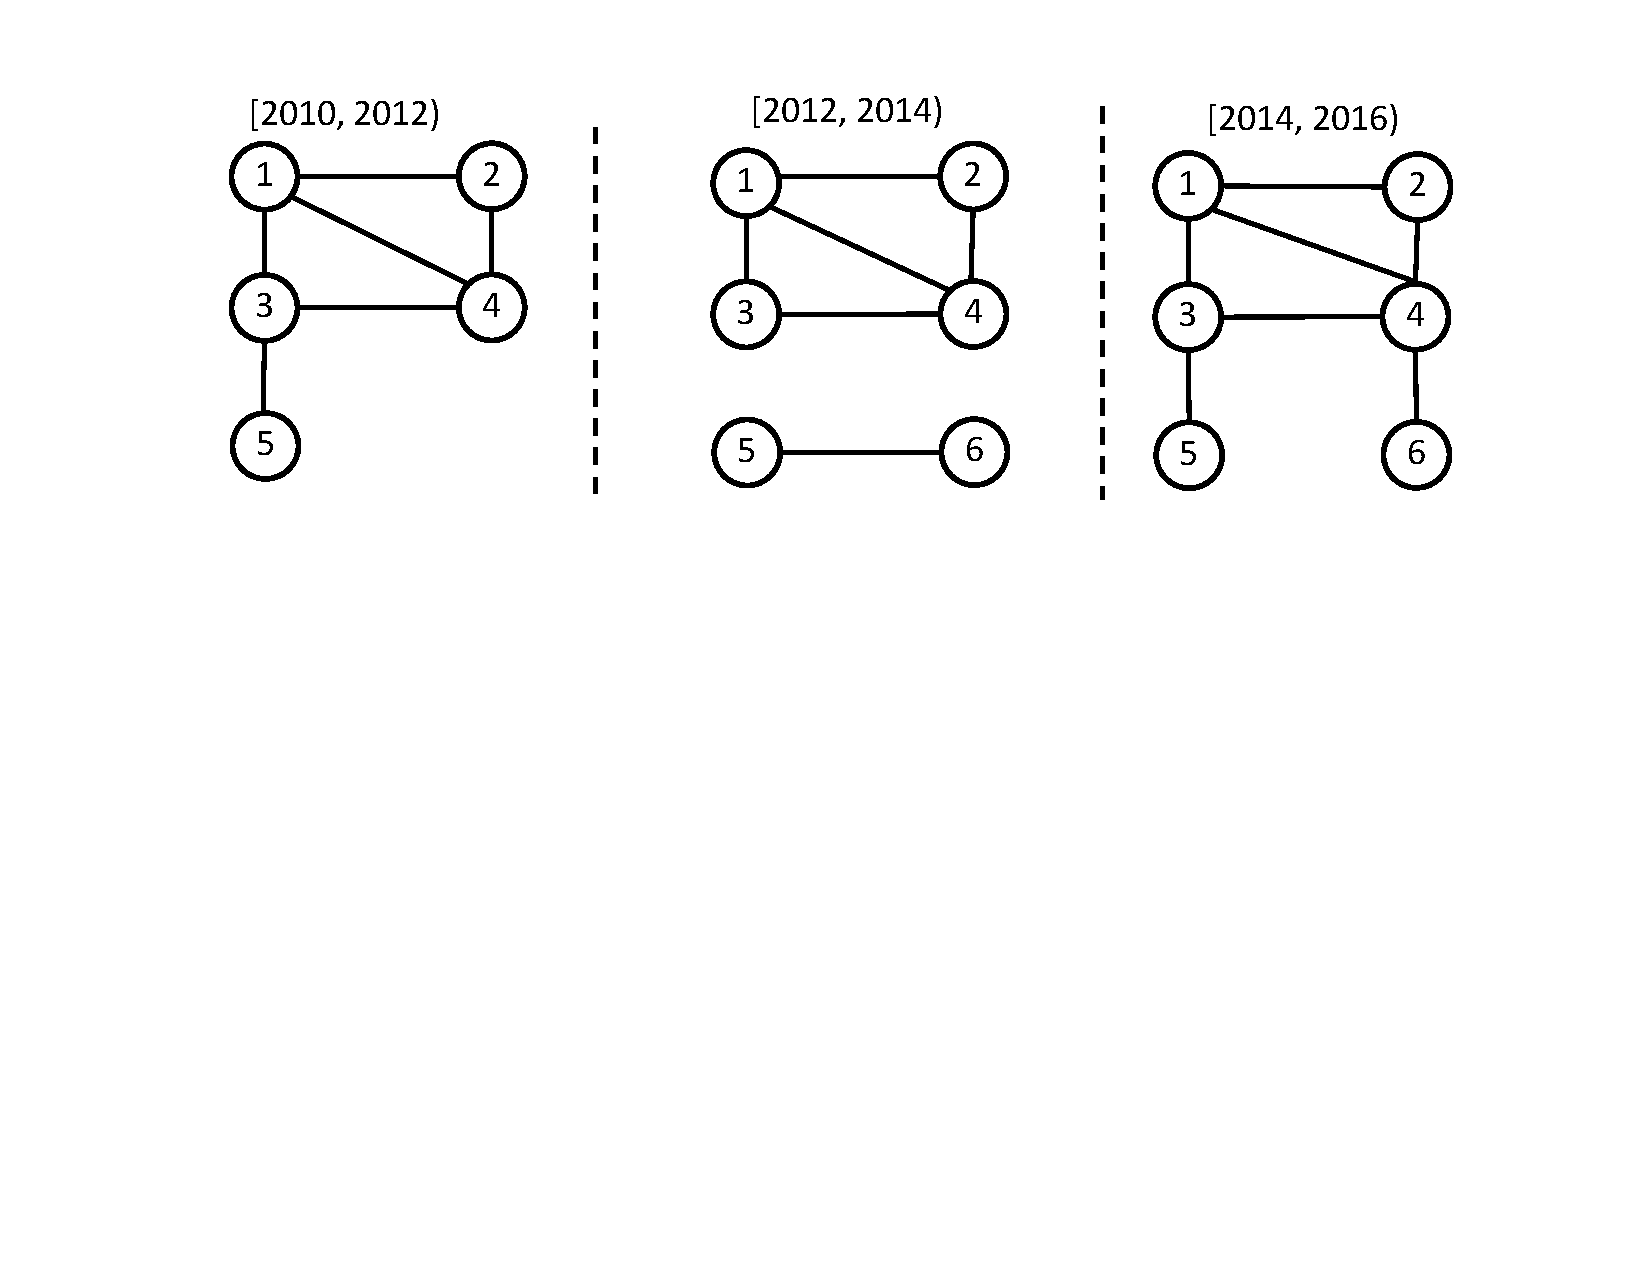
\includegraphics[width=2.5in]{figs/TGroupAny.pdf}
\vspace{-0.1in}
\caption{Result of query Q3 on T1.}
\label{fig:q3}
\end{figure}

Consider next query $Q4$, and its result in
Figure~\ref{fig:tg_all_any}.

\begin{small}
\begin{verbatim}
Q4: TSelect All V [vid, any(name), max(salary)] ; 
            Any E [vid1, vid2, sum(cnt)] 
    From    T1 
    TGroup  by 2 years
\end{verbatim}
\end{small}

The main difference between $Q4$ and $Q3$ is the \insql{All} modifier
associated with vertices in the \insql{TSelect} clause of $Q4$,
meaning that $\gamma^{V}_{vid, any(name), max(salary)}(\bigcap_{G_i
  \in {\cal G}} V(G_i))$ (Definition~\ref{def:sgroup}) is used to
aggregate vertices of snapshots in each 2-year group.  \insql{Any E}
states that the edges in the result correspond to the union of the
edges connecting the vertices.

\begin{figure}
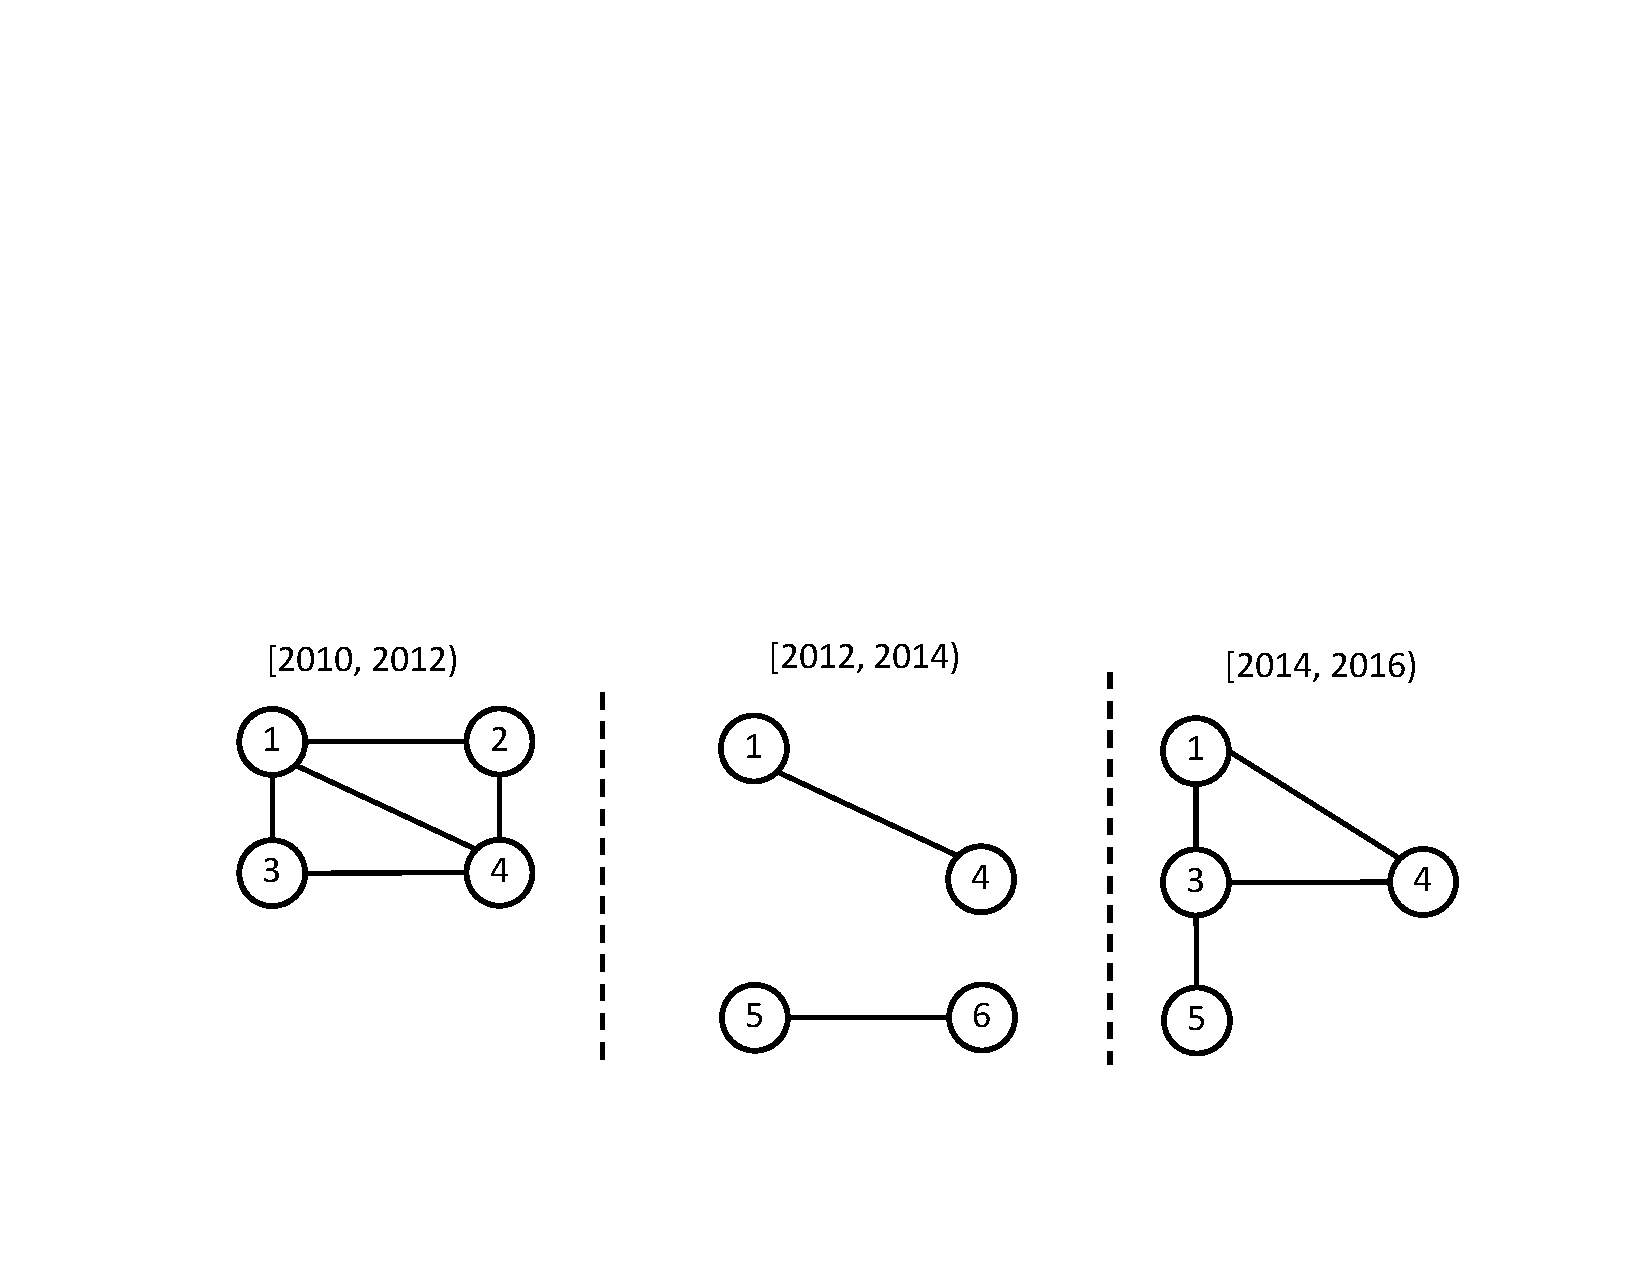
\includegraphics[width=2.5in]{figs/TGroupAllAny.pdf}
\caption{Result of query Q4 on T1.}
\label{fig:tg_all_any}
\vspace{-0.1in}
\end{figure}

$Q4$ illustrates another important feature of \ql, namely, aggregation
of values of non-key attributes of vertices and edges, which takes
place as part of structural aggregation.  We left available operations
unspecified in Definition~\ref{def:sgroup}, so as to keep structural
aggregation generic.  When used in scope of \insql{TGroup}, structural
aggregation operates over an ordered collection of snapshots.  \ql
makes the following aggregation operations available for ordered
snapshot collections: \insql{any}, \insql{first}, \insql{last},
\insql{min}, \insql{max}, \insql{sum}, \insql{count}, and
\insql{list}.

To illustrate, consider vertex and edge relations in
Figure~\ref{fig:3ve}, which correspond to the first three snapshots of
\insql{T1}.  Vertex 1 is present in both $[2010, 2011)$ and $[2011,
    2012)$ in \insql{T1}, and so is present in the snapshot $[2010,
      2012)$ of the result of $Q4$.  Vertex 1 has \insql{name='Alice'}
      in both snapshots, but different values for \insql{salary}.
      Therefore, taking any value of \insql{name} and the maximum
      \insql{salary} may be appropriate.  Operations \insql{first} and
      \insql{last} return the value corresponding to the earliest
      (resp. latest) occurrence of an attribute, while \insql{list}
      returns a collection of all attribute values.

Returning to query $Q3$, when aggregation of attribute values is not
specified explicitly, \insql{any} is used as the default for non-key
attributes.  That is, the \insql{TSelect} clause of $Q3$ is short-hand
for \insql{TSelect Any V[vid, any(name), any(salary)] ;} 
\insql{Any E[vid1, vid2, any(cnt)]}.

{\bf Temporal join.} We will now present two binary operators of \ql
that join together \tg relations, and will illustrate them using
\insql{T1} (Figure~\ref{fig:tg}) and \insql{T2}
(Figure~\ref{fig:tg_t2}).  Query $Q5$ computes temporal intersection
of \insql{T1} and \insql{T2}.  We require that \insql{T1} and
\insql{T2} be union-compatible, as per Definition~\ref{def:tuc}.  The
result of this query is in Figure~\ref{fig:q5}. 

\begin{small}
\begin{verbatim}
Q5:  TSelect   Any V; Any E
     From      T1 TAnd T2
\end{verbatim}
\end{small}

\begin{figure}
\centering
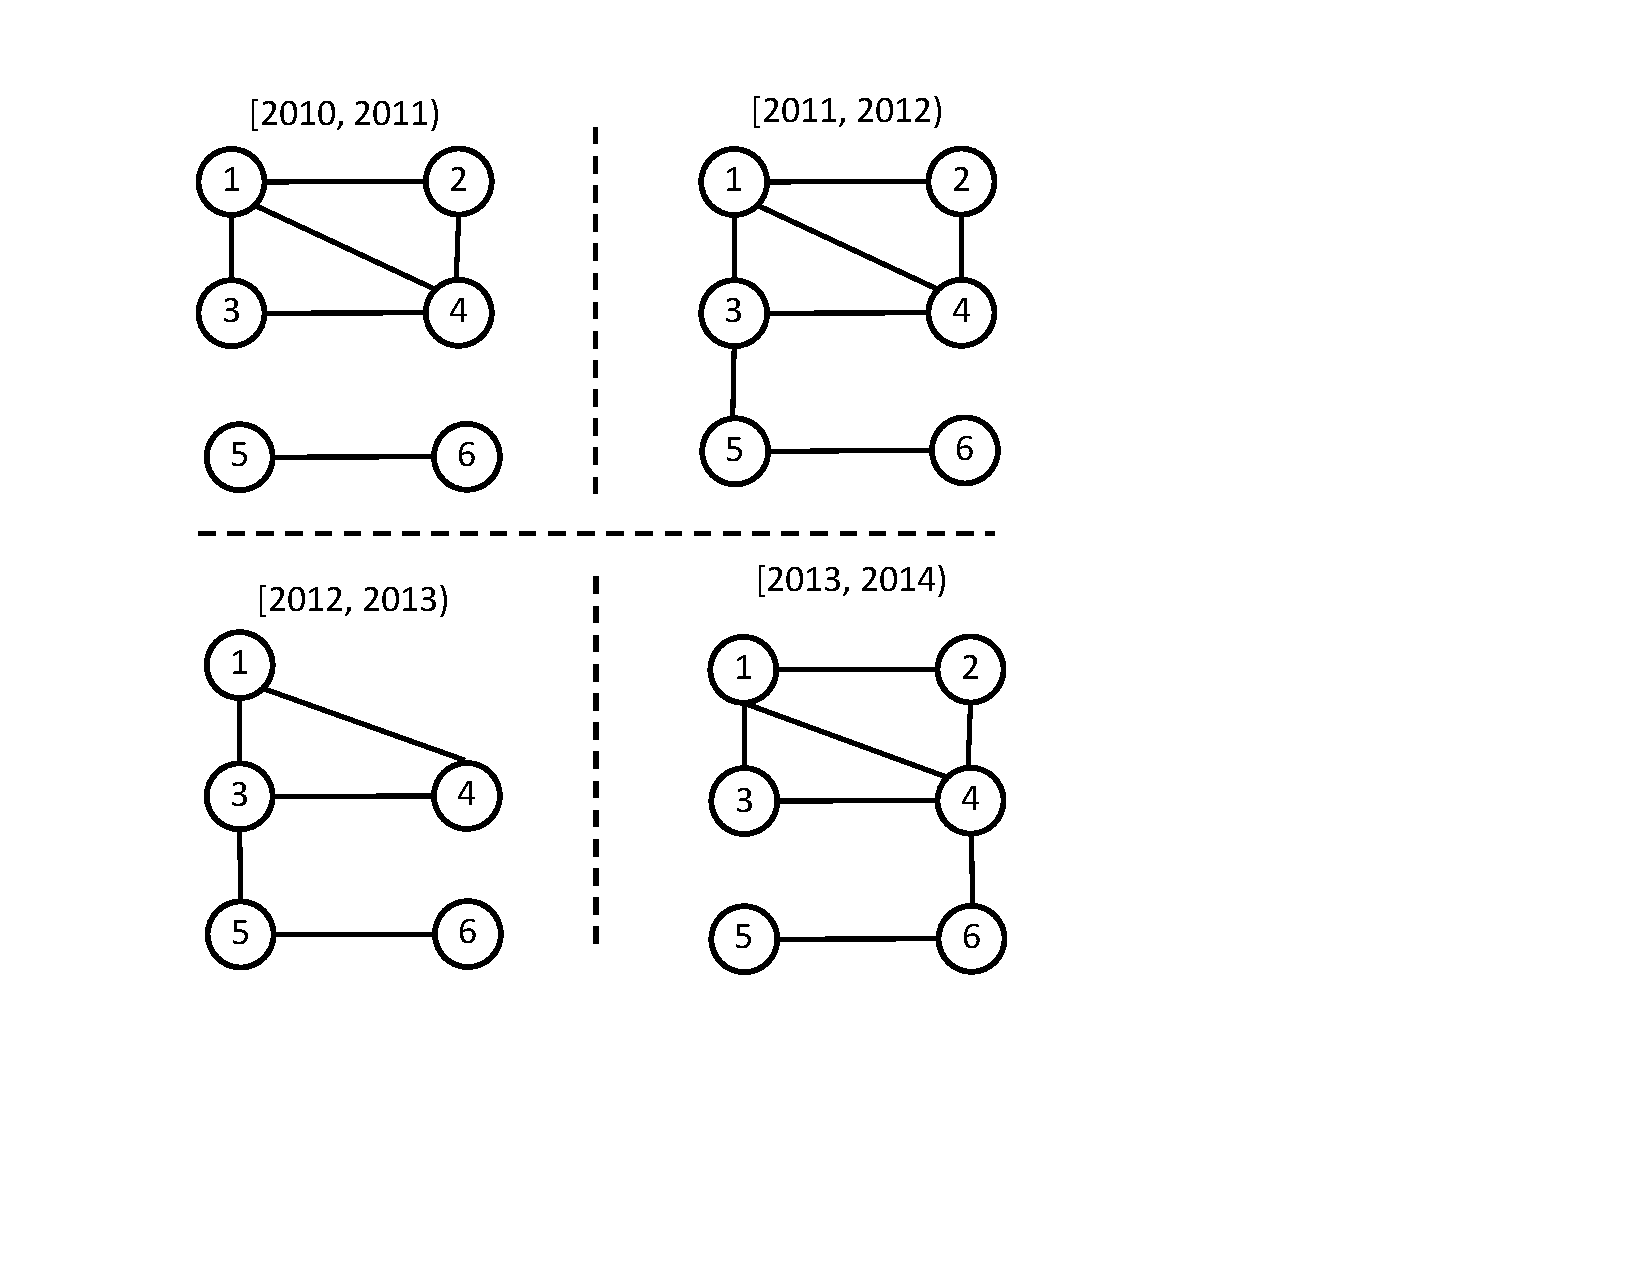
\includegraphics[width=2.8in]{figs/q5.pdf}
\caption{Result of query Q5.}
\vspace{-0.1in}
\label{fig:q5}
\end{figure}

Temporal schema of the result is computed according to
Definition~\ref{def:tseqand}, and corresponds to a sequence with
$P.start = 2010$, $P.end=2014$ and $P.size=4$.  Note the use of
\insql{Any V} and \insql{Any E} in the \insql{TSelect} clause.  This
is another example of structural aggregation
(Definition~\ref{def:sgroup}), now as part of \insql{TAnd}.  The
modifiers \insql{Any} and \insql{All} have the same meaning here as
for \insql{TGroup}, specifying that, a vertex (resp. edge) will be
present in a snapshot in the result if it is present in at least one
corresponding snapshot of \insql{T1} or \insql{T2}.  

An important difference is that, for \insql{TAnd} and \insql{TOr},
structural aggregation operates on unordered collections of snapshots,
with at most two snapshots per group.  \ql makes the following
aggregation operations available for unordered snapshot collections:
\insql{any}, \insql{min}, \insql{max}, \insql{sum}, \insql{count}, and
\insql{list}.  Note that, unlike for \insql{TGroup}, \insql{first} and
\insql{last} are unavailable here, and that \insql{any} is still the
default.

Consider next query $Q6$ that computes temporal union of \insql{T1}
and \insql{T2}.  The result of this query is shown in
Figure~\ref{fig:q6}.

\begin{small}
\begin{verbatim}
Q6:  TSelect   All V[vid, pagerank() as pr]; 
               Any E[vid1, vid2, sum(cnt)]
     From      T1 TOr T2
\end{verbatim}
\end{small}

\begin{figure}
\centering
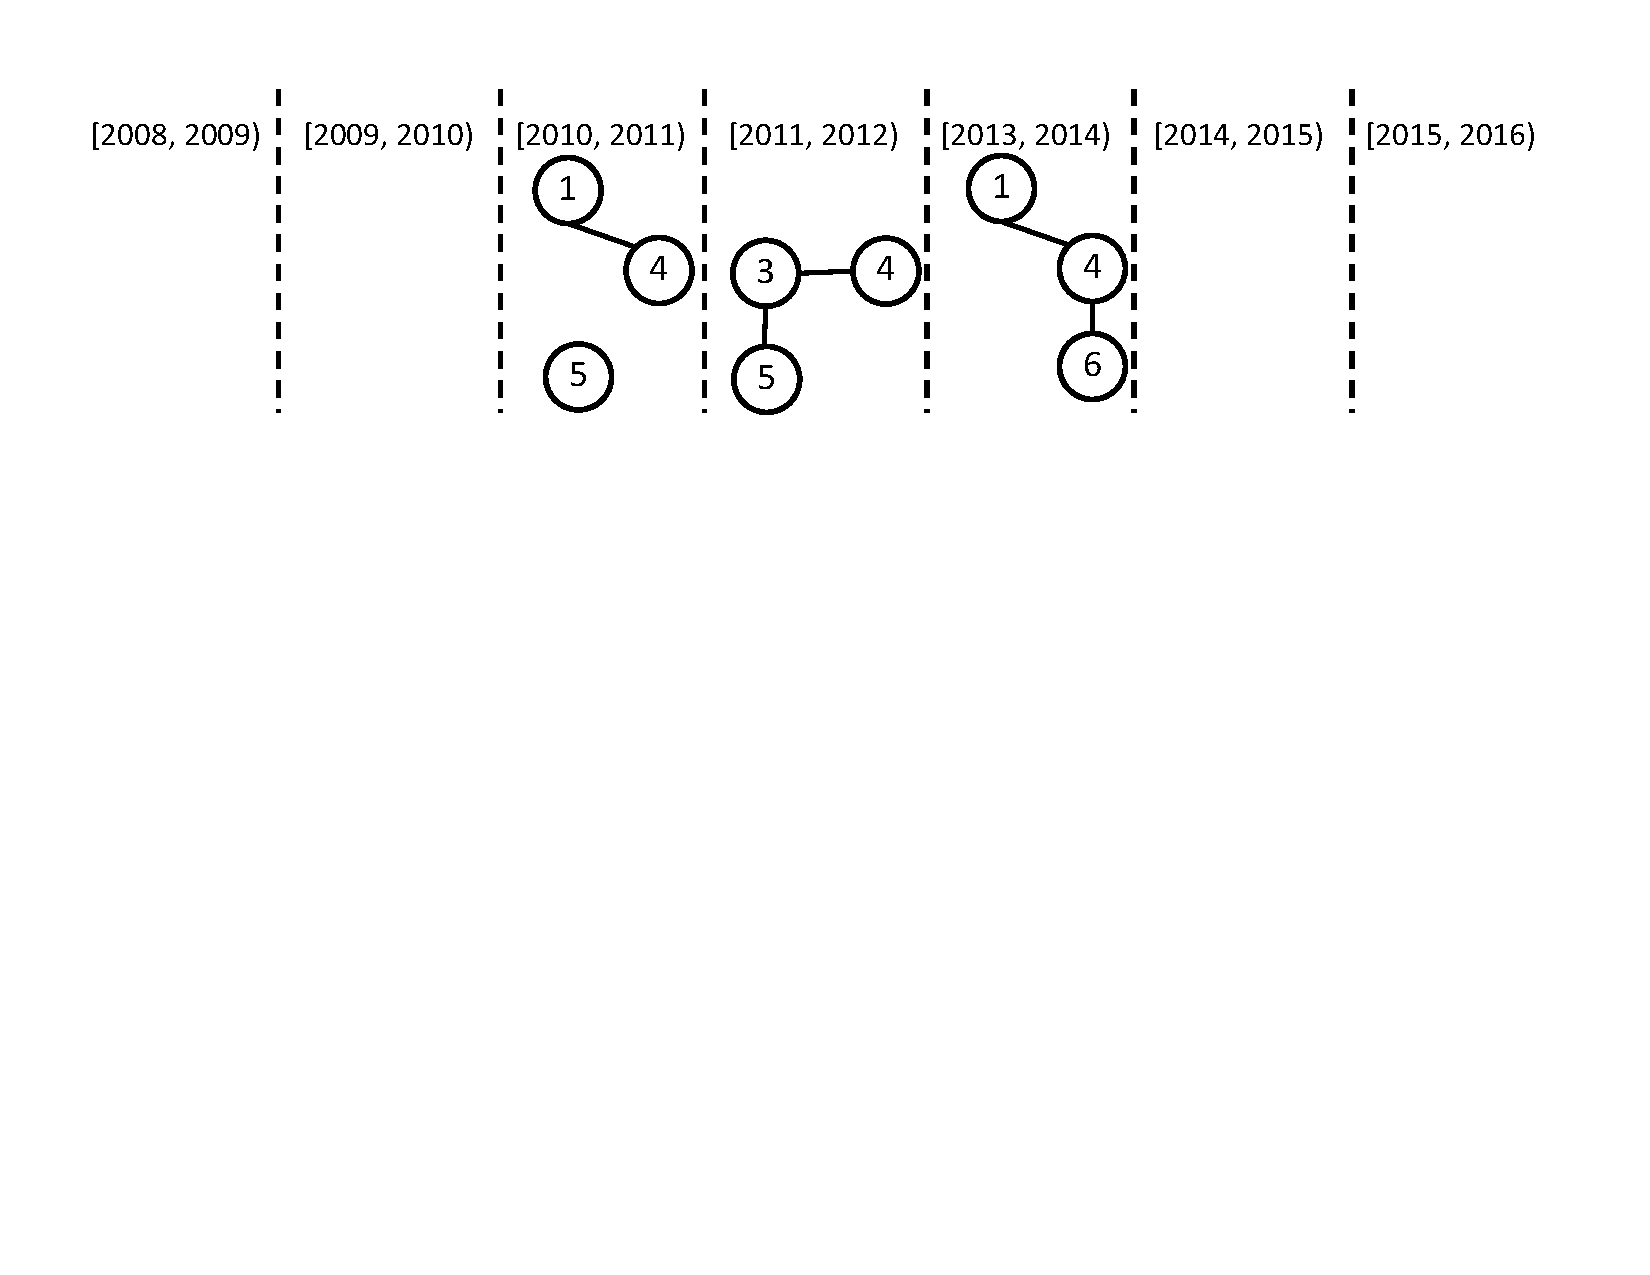
\includegraphics[width=3.4in]{figs/q6.pdf}
\vspace{-0.1in}
\caption{Result of query Q6.}
\label{fig:q6}
\vspace{-0.1in}
\end{figure}

Temporal schema of the result is computed according to
Definition~\ref{def:tseqor}, and corresponds to a sequence with
$P.start = 2008$, $P.end=2016$ and $P.size=8$.  Further, observe the
use of projection (non-key attributes of \insql{V} are not retained),
of an analytic function \insql{pagerank()}, and of the aggregation
operation \insql{sum} applied to the edge attribute \insql{cnt}.

\subsection{Complex queries}
\label{sec:example:complex}

{\bf Order of operators.} So far we illustrated individual operators
of \ql.  Now we will show how multiple operators can be combined in a
single query.  The logical order of evaluation of a \ql query without
nesting is as follows:

\begin{enumerate}
\item Temporal selection in the \insql{TWhere} clause;
\item Temporal join (\insql{TAnd} and \insql{TOr}) in the \insql{From}
  clause;
\item Temporal aggregation in the \insql{TGroup} clause;
\item Projection, computation of attribute aggregates and analytic
  functions.
\end{enumerate}

While the logical order of operations is predetermined, we will see in
Section~\ref{sec:sys:optimization} that some operators can be
reordered without affecting the result (but with potential differences
in performance), while others cannot.  

Consider $Q7$ below, with result shown in Figure~\ref{fig:q7}. $Q7$
first executes temporal selection on each \insql{T1} and \insql{T2}.
(Note that when temporal conditions in the \insql{TWhere} clause are
not qualified, they are applied to all \tgs in the \insql{From}
clause.)  Next, $Q7$ computes temporal intersection of \insql{T1} and
\insql{T2}, and then temporally aggregates the resulting \tg by 2
years.  Finally, \insql{pagerank()} is computed for each vertex in the
result.

\begin{small}
\begin{verbatim}
Q7:  TSelect Any V [vid, pagerank() as pr] ; 
             Any E [vid1, vid2] 
     From    T1 TAnd T2 
     TWhere  Start >= 2012 And End < 2014 
     TGroup  by 2 years
\end{verbatim}
\end{small}

\begin{figure}
\centering
\begin{minipage}{1.6in}
  \centering
  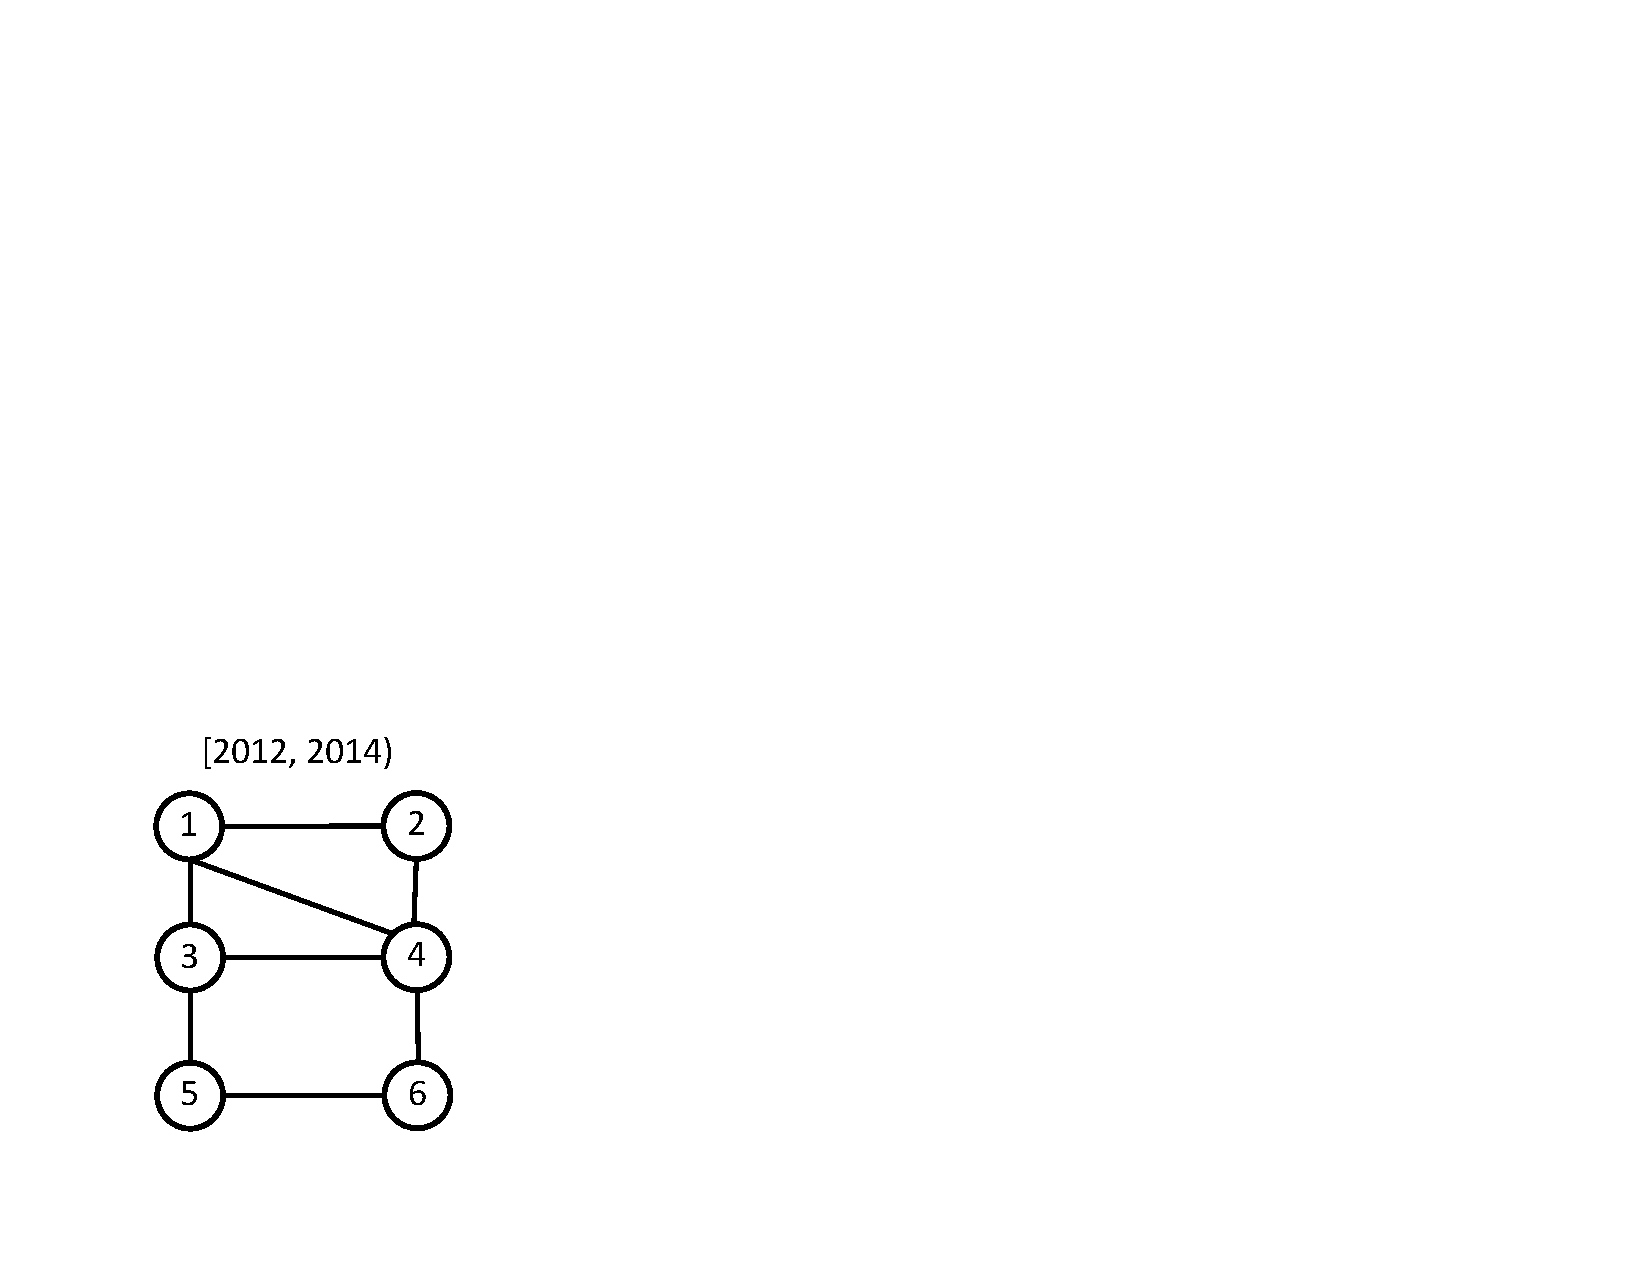
\includegraphics[width=0.8in]{figs/q7.pdf}
\vspace{-0.1in}
  \caption{Result of Q7.}{}
\vspace{-0.1in}
  \label{fig:q7}
\end{minipage}%
\begin{minipage}{1.6in}
  \centering
  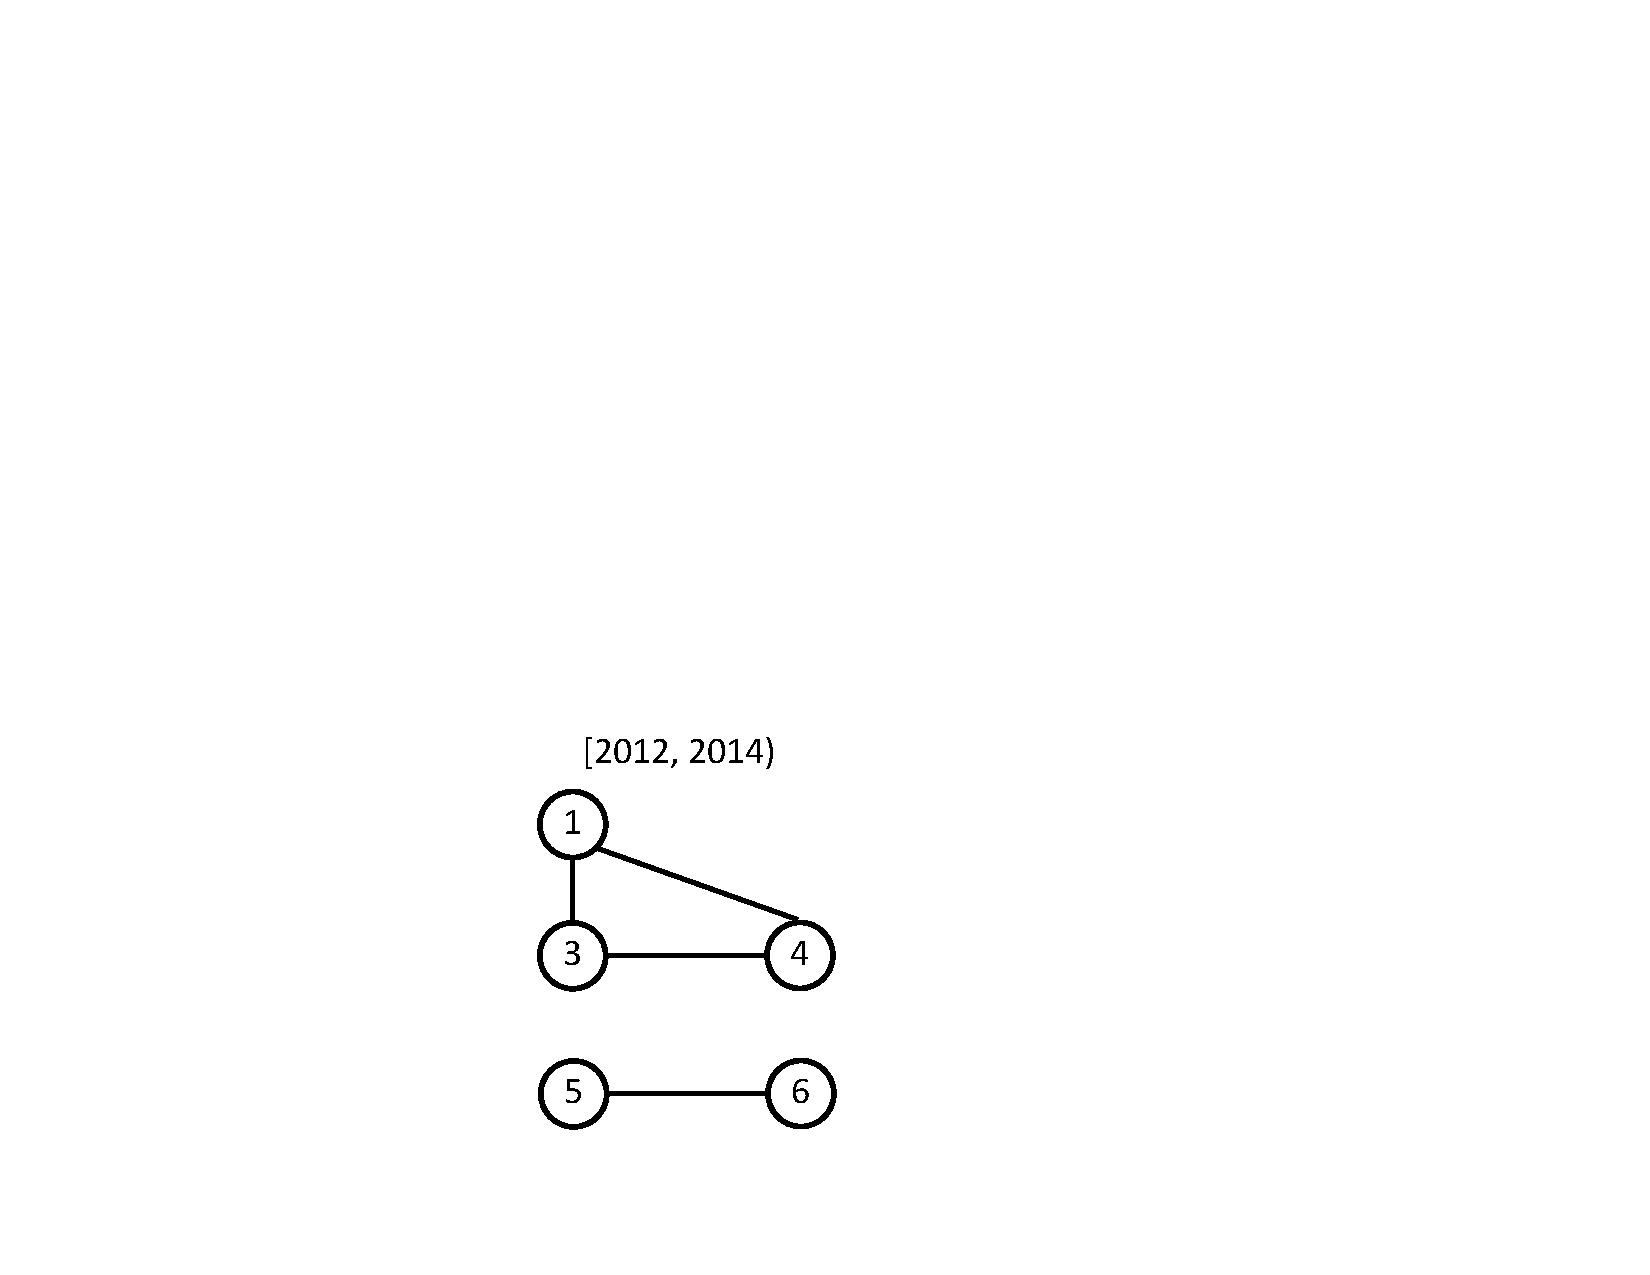
\includegraphics[width=0.8in]{figs/q8.pdf}
\vspace{-0.1in}
  \caption{Result of Q8.}{}
  \label{fig:q8}
\vspace{-0.1in}
\end{minipage}
\end{figure}

Observe that \insql{TAnd} and \insql{TGroup} use the same
specification in the \insql{TSelect} clause, that is, we cannot
decouple structural aggregation behavior of the two operations in a
query of this kind.

Consider next query $Q8$ that is similar to $Q7$, but uses nesting to
decouple structural aggregation of \insql{TSelect} from that of
\insql{TGroup}. The result of executing $Q8$ is shown in
Figure~\ref{fig:q8}.

\begin{small}
\begin{verbatim}
Q8:  TSelect   All V [vid, pagerank() as pr];
               All E [vid1, vid2]
     From      ( TSelect Any V [vid] ; 
                         Any E [vid1, vid2]
                 From    T1 TAnd T2
                 TWhere  Start >= 2012 
                 And     End < 2014 )
     TGroup    by 2 years
\end{verbatim}
\end{small}

{\bf Trend analytics.} We argued in the introduction that it is
important to support analysis of trends in evolving graphs.  The \ql
query language makes this sophisticated analysis possible.  Query $Q9$
illustrates this; it invokes the snapshot analytic \insql{pagerank()}
on \insql{T1}, and then computes the trend in these values across all
snapshots.

\begin{small}
\begin{verbatim}
Q9:  TSelect Any V[vid, trend(pr) as tr, max(pr) as mx];
             Any E[vid1, vid2]  
     From    ( TSelect V[vid, pagerank() as pr];   
                       E[vid1, vid2]
               From    T1 )
     TGroup  by Size
\end{verbatim}
\end{small}

Consider the use of the {\em trend analytic} function
\insql{trend(pr)}, which aggregates the sequence of PageRank scores of
each vertex.  In our implementation we use a common definition of
\insql{trend}: compute the slope of the least squares line using
linear regression, making an adjustment when a vertex value is
missing.  While this is the only trend analytic we currently support,
we are working on an API that will allow developers to implement
custom trend analytics, taking attributes of both atomic and complex
type as input, and computing a value of either an atomic or a complex
type.

We invoke \insql{trend(pr)} alongside \insql{max(pr)} in $Q9$, to
highlight the difference between a trend analytic and value
aggregation.  Syntactically, the two look the same, but the difference
is that \insql{max(pr)} does not account for the temporal order of
values being aggregated, while \insql{trend(pr)} does.  Based on this
distinction, it is not meaningful to invoke a trend analytic when
structural aggregation is due solely to temporal join (\insql{TAnd})
or (\insql{TOr}), but only as part of a query that does temporal
aggregation (\insql{TGroup}).

Finally, recall from our discussion of temporal aggregation that
\insql{TGroup by Size} produces a 1-snapshot \tg.  It is convenient,
although not required, to use this feature in a query such as $Q9$,
since a temporal trend may be computed over a window of any size.

\subsection{Loading data and inspecting results}
\label{sec:example:loadshow}

{\bf Loading filesystem data.  Views.}  Queries $Q1$ through $Q9$
refer to \tg variables in the \insql{From} clause.  The value of a \tg
variable is assigned by the \insql{define view} statement.  This value
may be loaded from the file system, as in query $Q10$, or it may
correspond to a view, as in query $Q11$.

\begin{small}
\begin{verbatim}
Q10:  Create TView T1 as 
        (TSelect V[vid:int, name:str, salary:int]; 
                 E[vid1:int, vid2:int, cnt:int]
         From    path/to/directory)
\end{verbatim}
\end{small}

\begin{small}
\begin{verbatim}
Q11:  Create TView T4 as (TSelect V; E
         From    T1
         TWhere  Start >=  2010)
\end{verbatim}
\end{small}

Note that when data is loaded into a \tg variable from the file
system, as in $Q10$, the \insql{TSelect} clause must specify the
structural schema.  When a \tg variable takes on a value computed by a
query, its structural schema is determined by the query result.  In
$Q11$, the structural schema of the view \insql{T4} is the same as
that of \insql{T1}.

{\bf Inspecting results with SQL.}  Suppose that the result of $Q9$ is
assigned to \insql{T5}, with the structural schema
V(\underline{vid}:int, tr:float, mx:float) ; E(\underline{vid1}:int,
\underline{vid2}:int).  The SQL query below shows \insql{vid}
and \insql{tr} values of 20 vertices with the most significantly
increasing \insql{pagerank} trend.

\begin{small}
\begin{verbatim}
Q12:  Select   VF.vid, VF.tr  
      From     T5.toVerticesFlat() as VF
      Order by tr
      Limit    20
\end{verbatim}
\end{small}

The important part of \insql{Q12} is the use of
\insql{T5.toVerticesFlat()} in the \insql{From} clause.  This is a
multi-step operation provided by the \ql framework, which starts by
collecting all vertices in the union of snapshots of \insql{T5} into a
single nested vertex collection, and associating \underline{vid} with
a time-indexed map of vertex attributes.  Next, the nested collection
is flattened into \insql{VF} (\underline{vid}:int,
\underline{start}:date, \underline{end}:date, tr:float, mx:float).
\insql{VF} can be used in SQL queries.  The \ql framework also
provides an operation that returns a flattened collection of edges,
called \insql{toEdgesFlat()}.




